\documentclass[beamer=true]{standalone}
\usepackage{../../preamblesnotes}

\begin{document}
\settitle{透鏡\\Lenses}{光學第四課(I)}{周末班}

\begin{frame}{透鏡的種類 Types of lens}
    \begin{itemize}
        \item 凸透鏡:中心比邊緣厚\\Convex lens: thicker at centre
        \item 凹透鏡:中心比邊緣薄\\Concave lens: thinner at centre
    \end{itemize}\bigskip
    \begin{figure}
        \centering
        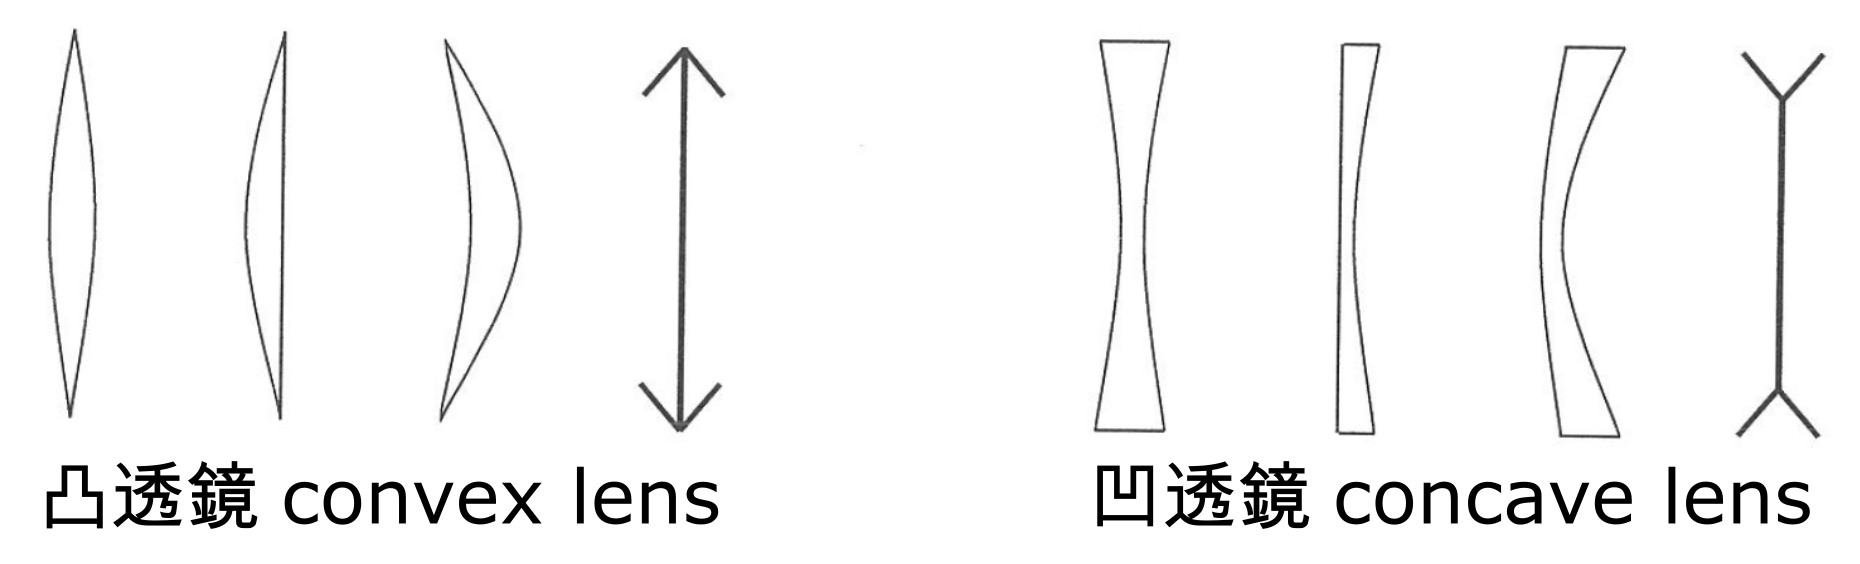
\includegraphics[width=1\linewidth]{assets/x1n98exu9198b12ec.png}
    \end{figure}

\end{frame}


\begin{frame}{凸透鏡Convex lens}
    \begin{figure}
        \centering
        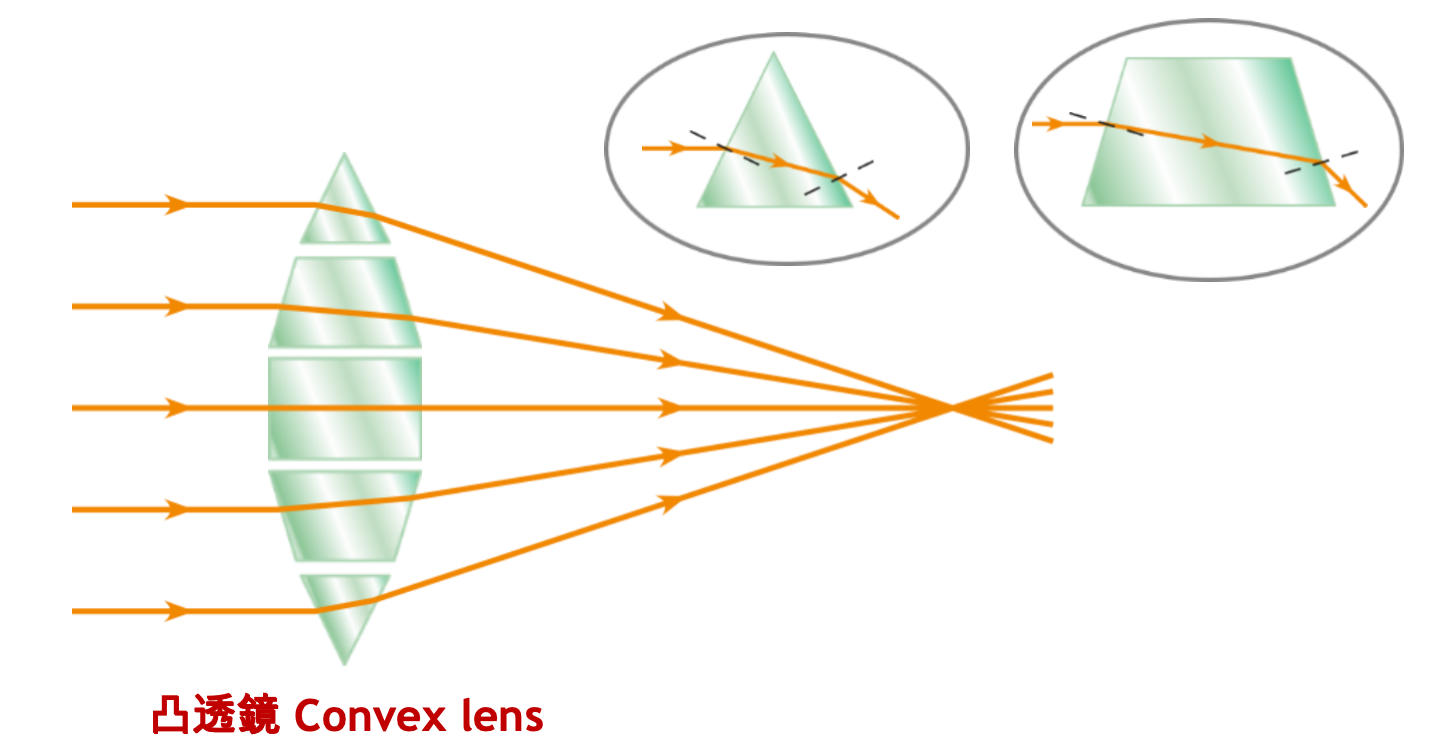
\includegraphics[width=1\linewidth]{assets/12d899d8b.png}
    \end{figure}
\end{frame}

\begin{frame}{凹透鏡Concave lens}
    \begin{figure}
        \centering
        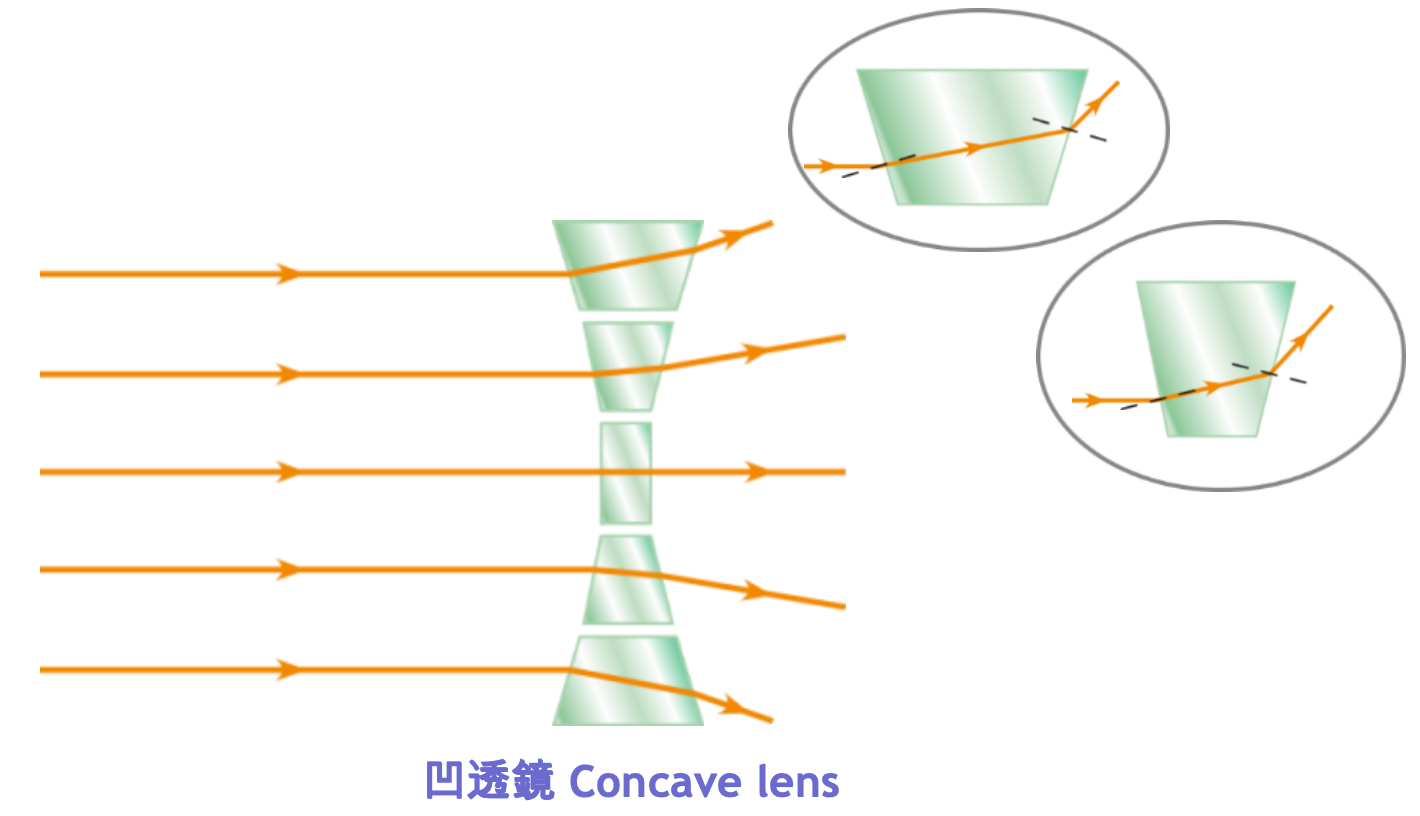
\includegraphics[width=1\linewidth]{assets/n8uxe892e.png}
    \end{figure}
\end{frame}

\begin{frame}{一些術語Terminology}
    \begin{figure}
        \centering
        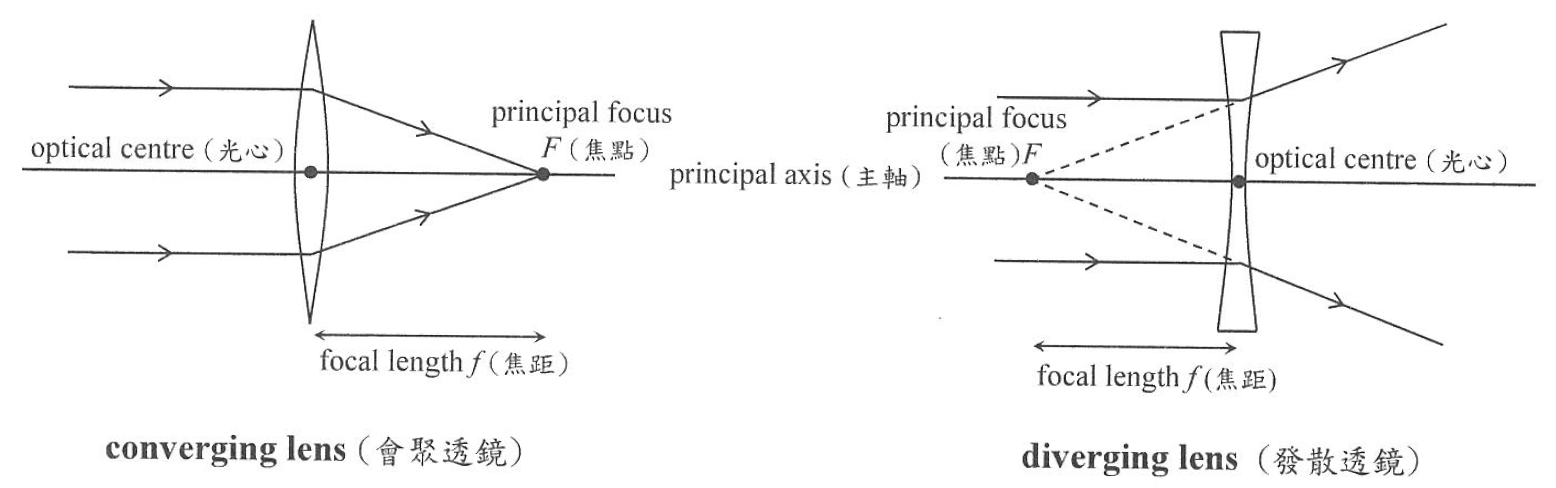
\includegraphics[width=1\linewidth]{assets/nxu98ru393n28urnc23.png}
    \end{figure}
\end{frame}

\begin{eg}
    如圖所示,通過將兩個透鏡X和Y放置在所示位置,可以將狹窄的平行光束轉換為更寬的平行光束。在以下組合中,選擇並正確安裝哪一組可以產生所需的效果?\\As shown in the diagram, a narrow parallel beam of light is converted to a wider parallel beam by placing two lenses X and Y in the positions shown. Which of the combinations below when correctly chosen and installed could produce the effect required?
    \begin{figure}
        \centering
        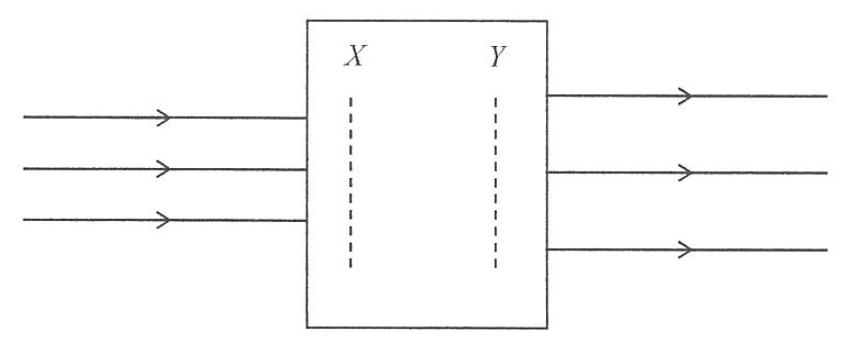
\includegraphics[width=0.75\linewidth]{assets/89ndu8n91b.png}


    \end{figure}
\end{eg}
\begin{eg}
    \begin{statements}
        \task [] \textbf{X}\tab \textbf{Y}
        \task 凸透鏡convex \tab 凹透鏡concave
        \task 凹透鏡concave \tab 凹透鏡concave
        \task 凹透鏡concave \tab 凸透鏡convex
    \end{statements}
    \begin{tasks}
        \task 只有(2) \tab (2) only
        \task 只有(3) \tab (3) only
        \task 只有(1)和(3) \tab (1) and (3) only
        \task 只有(2)和(3) \tab (2) and (3) only
    \end{tasks}
\end{eg}

\begin{frame}{光心Optical centre}
    % \begin{columns}
    %     \column{.5\textwidth}

    %     \column{.5\textwidth}
    % \end{columns}
    \begin{itemize}
        \item 若光線斜向射向光心 C,\\For a ray passing through C at an angle,
              \begin{itemize}
                  \item 出射光線的方向不變。\\its direction does not change.
                  \item 光線會出現旁向位移。\\it is displaced laterally.
              \end{itemize}
    \end{itemize}
    \begin{figure}
        \centering
        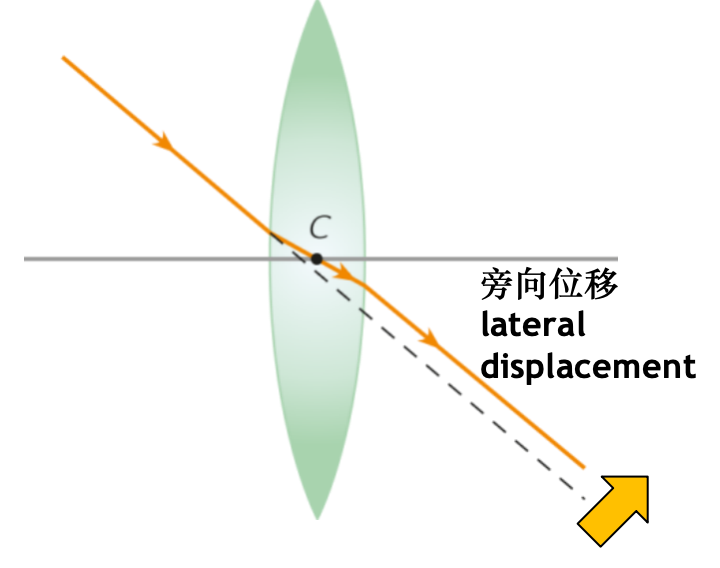
\includegraphics[width=0.5\linewidth]{assets/98ncu238uc9823rcc.png}


    \end{figure}
\end{frame}

\begin{frame}{光心Optical centre}
    \begin{itemize}
        \item 對於薄透鏡,我們可以忽略旁向位移的影響。\\The lateral displacement can be neglected for a thin lens.
    \end{itemize}
    \begin{figure}
        \centering
        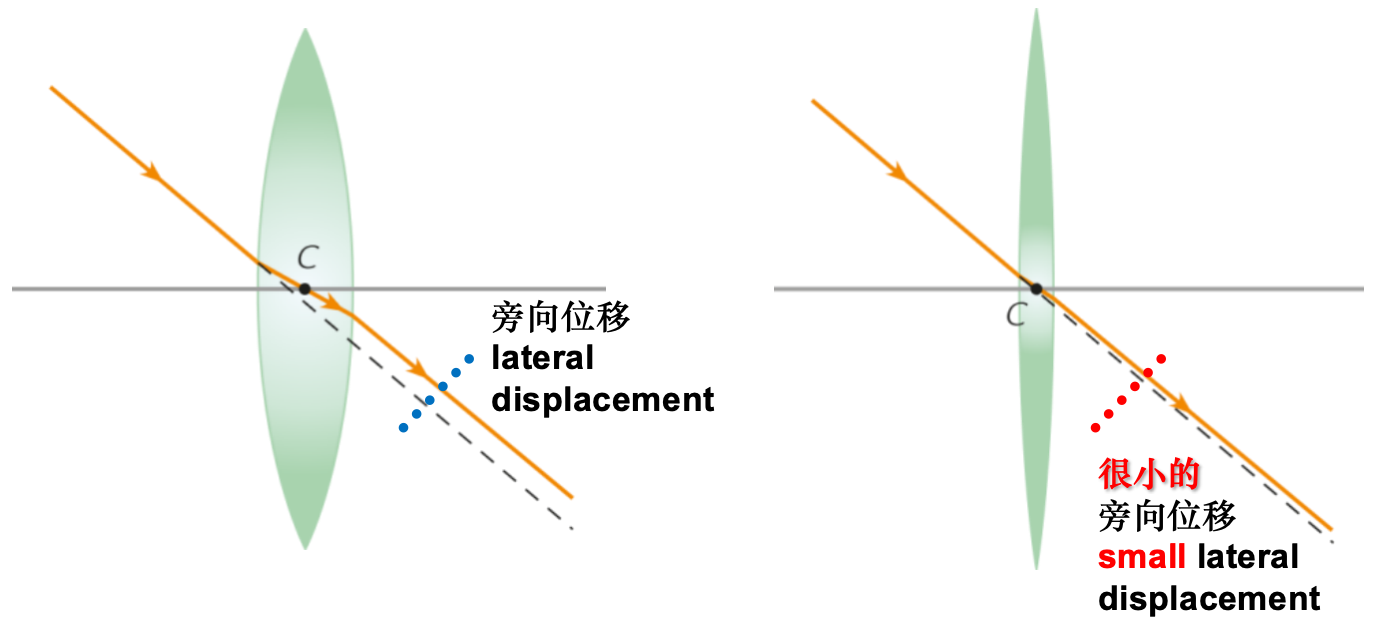
\includegraphics[width=1\linewidth]{assets/d9n823f.png}


    \end{figure}
\end{frame}

\begin{frame}{焦距Focal length}
    \begin{figure}
        \centering
        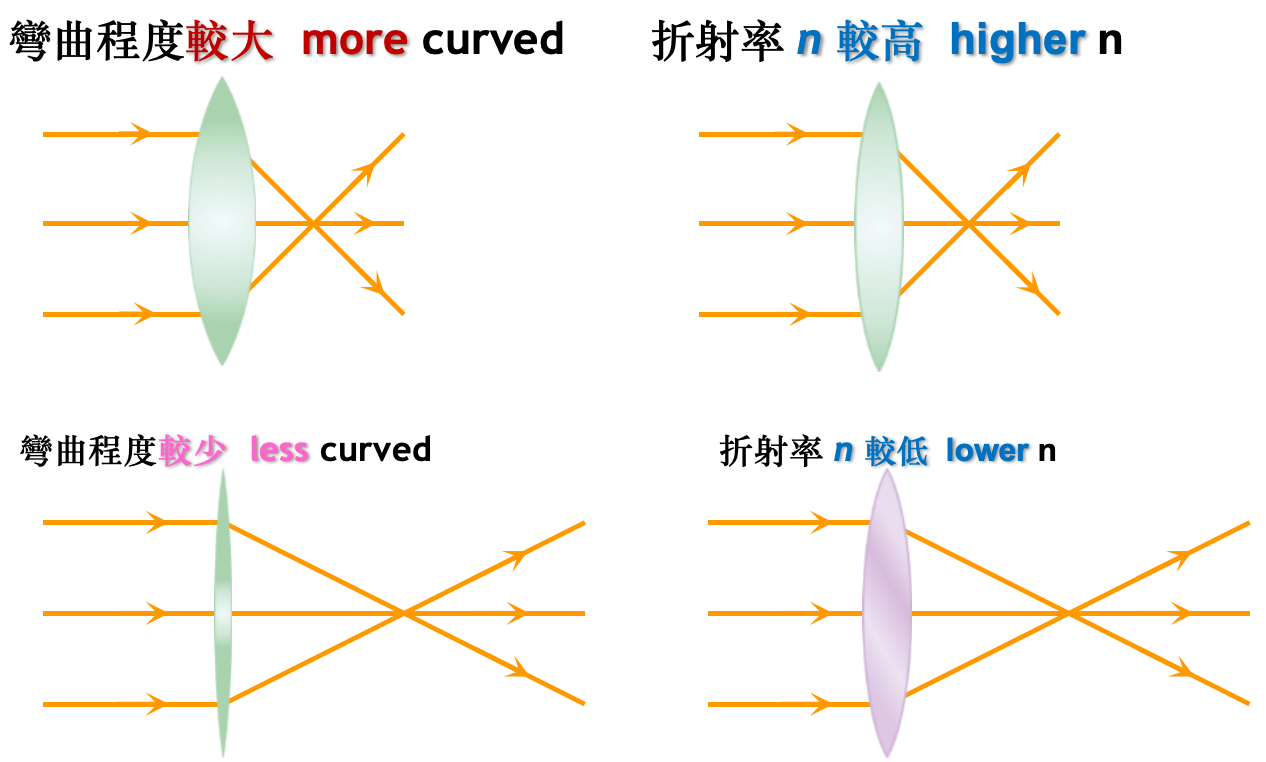
\includegraphics[width=1\linewidth]{assets/x91bey74r.png}


    \end{figure}
\end{frame}

\begin{frame}{焦距Focal length}
    \begin{itemize}
        \setlength{\itemsep}{0.6em}
        \item 要增加(凸透鏡或凹透鏡)焦距,我們可以\\To increase focal length (of both convex or concave lens), we can
              \begin{itemize}
                  \item 降低透鏡的厚度\\decrease the thickness of the lens
                  \item 降低透鏡材質的折射率\\decrease the refractive index of the material
              \end{itemize}
    \end{itemize}
\end{frame}

\section{rules}

\begin{frame}{凸透鏡的規則Rules for convex lens}
    \begin{itemize}
        \item [(1)] 光線直線通過光心。\\A light ray passes straight through the optical centre.
    \end{itemize}\bigskip

    \begin{figure}
        \centering
        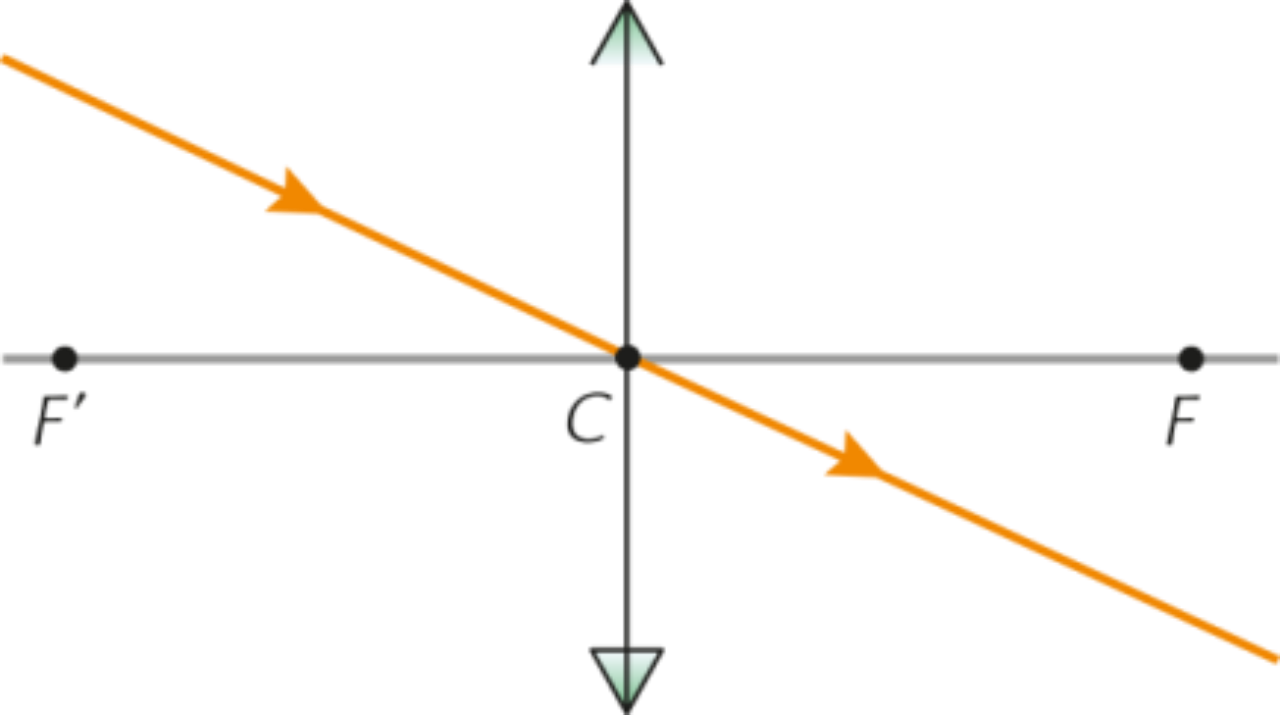
\includegraphics[width=0.5\linewidth]{assets/d112f2mage.png}


    \end{figure}
\end{frame}

\begin{frame}{凸透鏡的規則Rules for convex lens}
    \begin{itemize}
        \item [(2)] 平行於主軸的入射光線,通過透鏡後會穿過主焦點。\\An incident ray parallel to the principal axis bends towards the principal focus.
    \end{itemize}\bigskip
    \begin{figure}
        \centering
        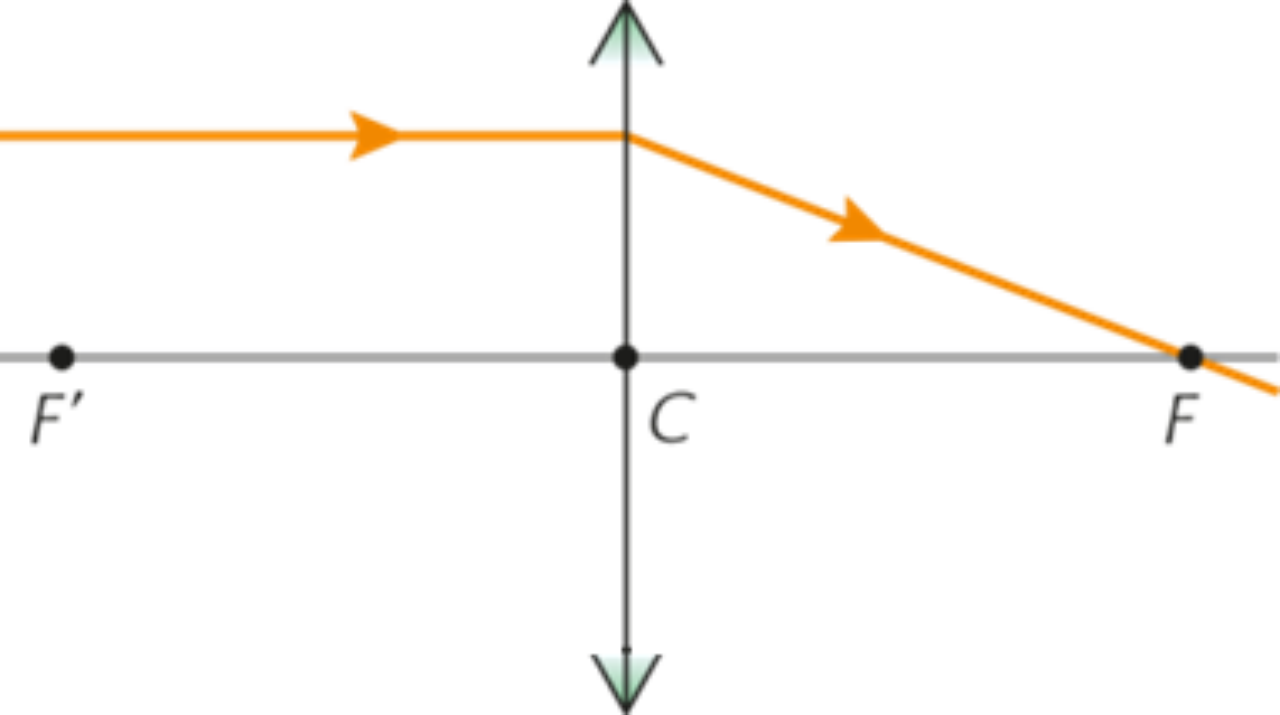
\includegraphics[width=0.5\linewidth]{assets/89nud89u298d.png}


    \end{figure}
\end{frame}

\begin{frame}{凸透鏡的規則Rules for convex lens}
    \begin{itemize}
        \item [(3)] 穿過主焦點的入射光線,通過透鏡後會平行於主軸。\\An incident ray passing through the principal focus becomes parallel to the principal axis.
    \end{itemize}\bigskip

    \begin{figure}
        \centering
        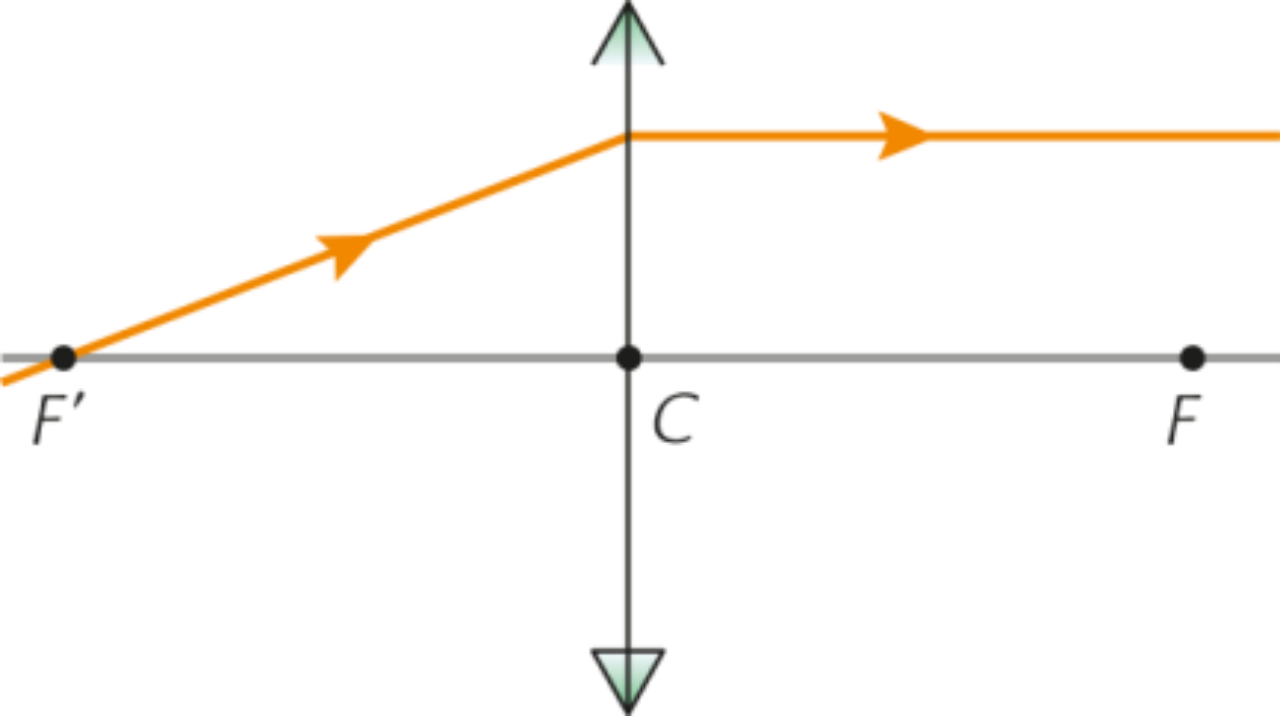
\includegraphics[width=0.5\linewidth]{assets/di0923in93i2e.png}


    \end{figure}
\end{frame}

\begin{frame}{凸透鏡的規則Rules for convex lens}
    \begin{itemize}
        \item 平行的多條光線必定在焦平面上聚焦。\\Multiple parallel rays must converge on the focal plane.
    \end{itemize}
    \begin{figure}
        \centering
        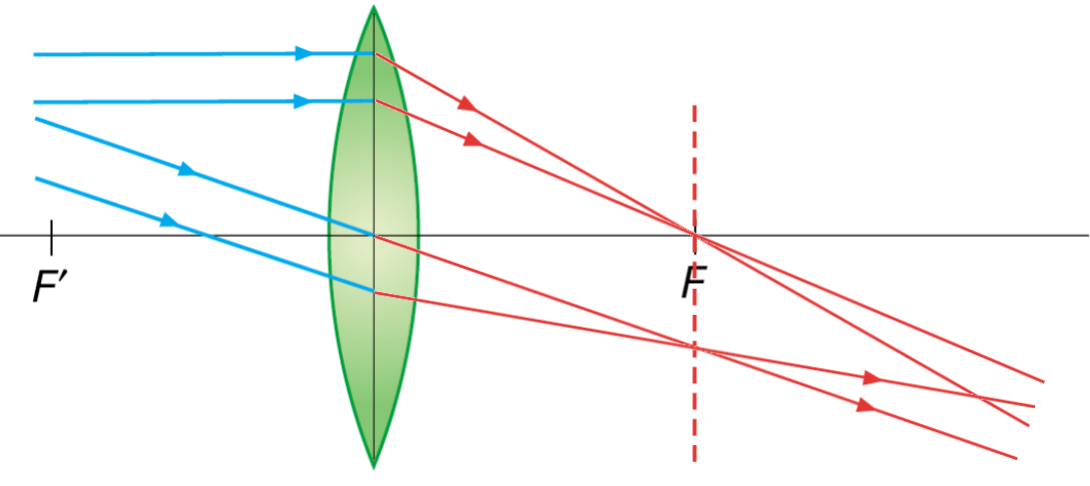
\includegraphics[width=0.85\linewidth]{assets/d892u3nd98n32ge.png}


    \end{figure}
\end{frame}

\begin{frame}{凹透鏡的規則Rules for concave lens}
    \begin{itemize}
        \item [(1)] 光線直線通過光心。\\A light ray passes straight through the optical centre.
    \end{itemize}\bigskip
    \begin{figure}
        \centering
        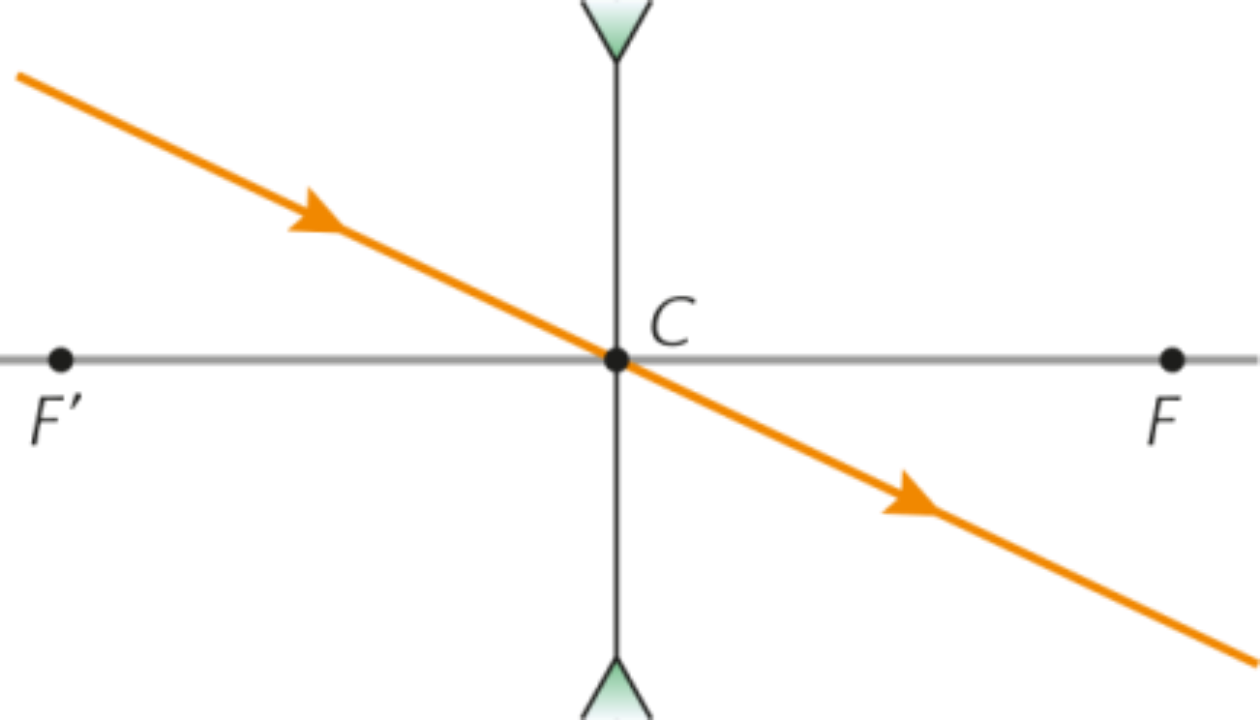
\includegraphics[width=0.5\linewidth]{assets/ima8e9nu1289e9nue9812ge.png}


    \end{figure}
\end{frame}


\begin{frame}{凹透鏡的規則Rules for concave lens}
    \begin{itemize}
        \item [(2)] 平行於主軸的入射光線,通過透鏡後看似從主焦點 F' 發散出來。\\An incident ray parallel to the principal axis appears to diverge from the principal focus F' upon leaving the lens.
    \end{itemize}\bigskip
    \begin{figure}
        \centering
        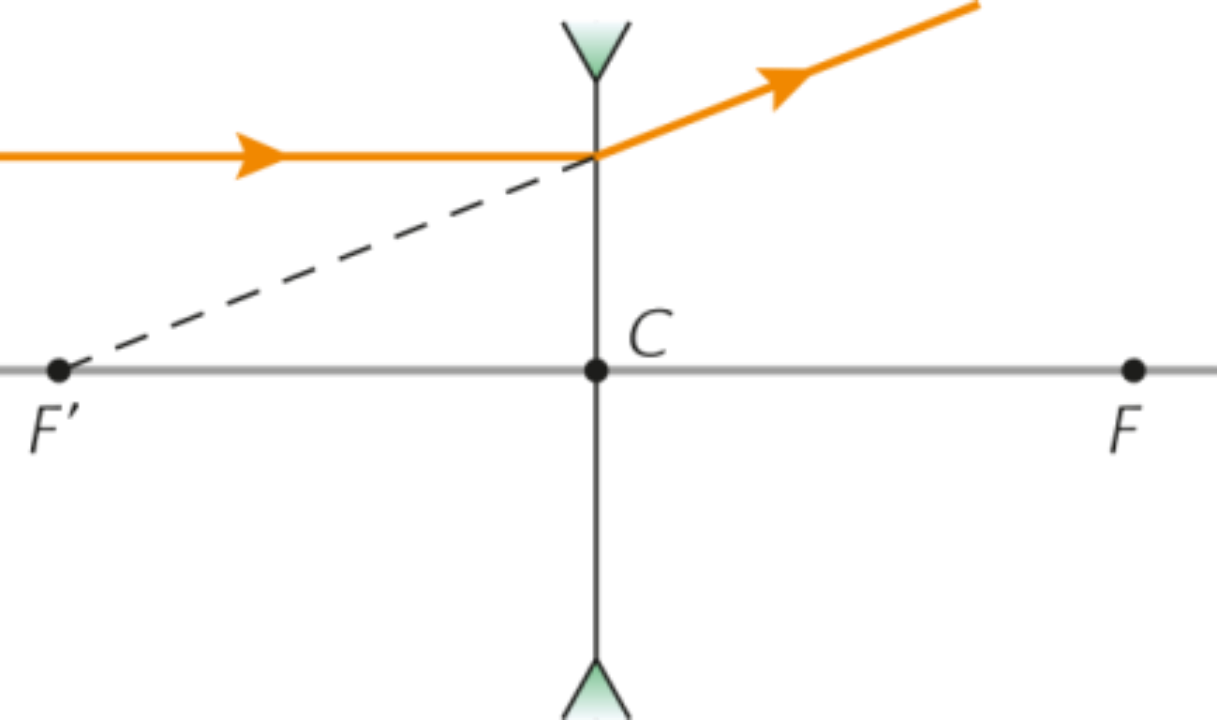
\includegraphics[width=0.5\linewidth]{assets/dun98dud98n98322d3.png}


    \end{figure}
\end{frame}

\begin{frame}{凹透鏡的規則Rules for concave lens}
    \begin{itemize}
        \item [(3)] 指向主焦點 的入射光線,通過透鏡後會平行於主軸。\\An incident ray directed towards the principal focus becomes parallel to the principal axis.
    \end{itemize}\bigskip
    \begin{figure}
        \centering
        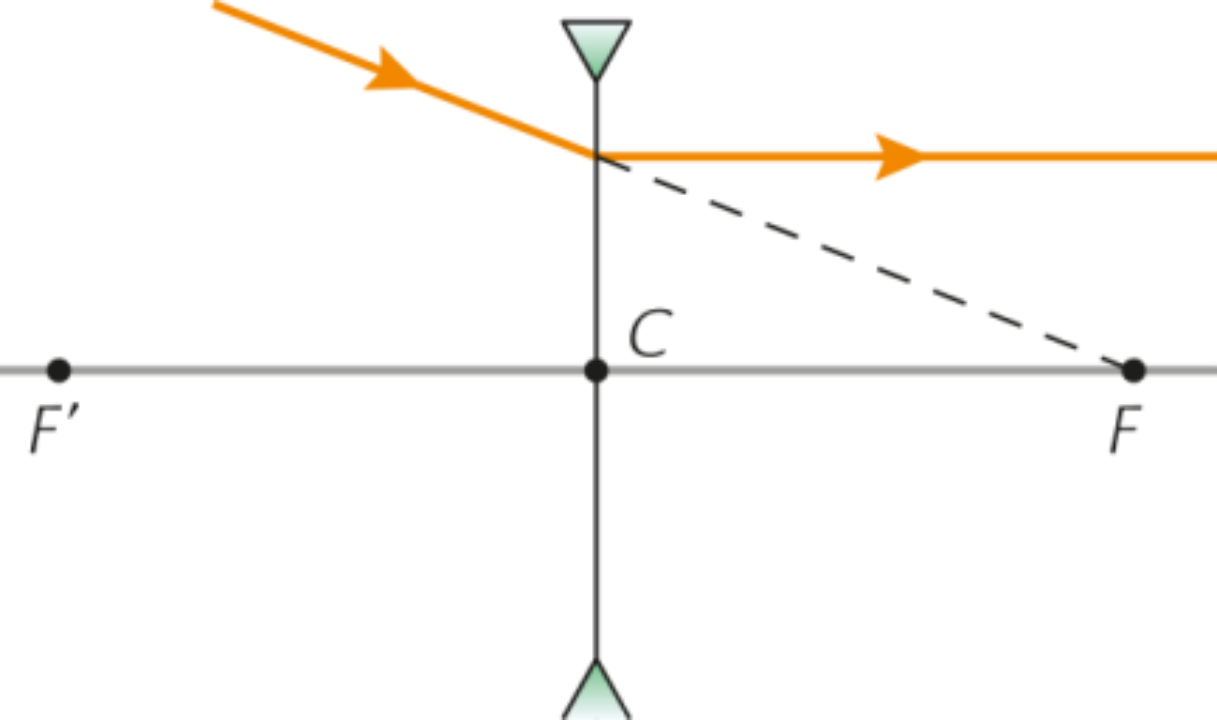
\includegraphics[width=0.5\linewidth]{assets/d2dn902332ige.png}
    \end{figure}
\end{frame}

\begin{frame}{凹透鏡的規則Rules for concave lens}
    \begin{itemize}
        \item 平行的光線貌似從焦平面發散出去。\\Parallel rays appear to diverge from a point on the focal plane.
    \end{itemize}
    \begin{figure}
        \centering
        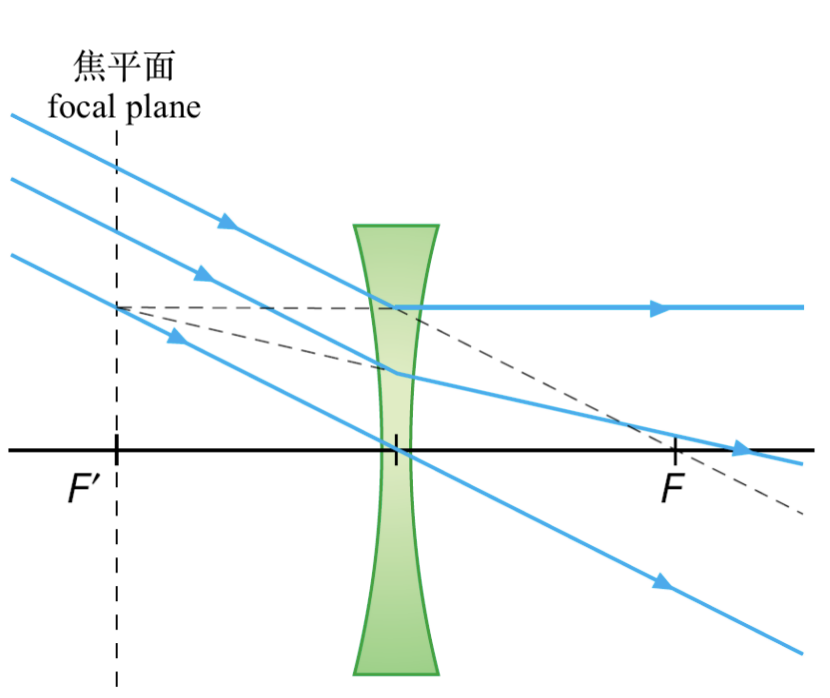
\includegraphics[width=0.65\linewidth]{assets/d0un209d2ungff.png}


    \end{figure}
\end{frame}

\section{examples}

\begin{eg}
    光線斜射到一個凸透鏡上。哪一個最能代表光線的路徑,X、Y還是Z?\\A light ray is incident on a convex lens. Which one best represents the path of the light ray, X, Y or Z?
    \bigskip
    \begin{figure}
        \centering
        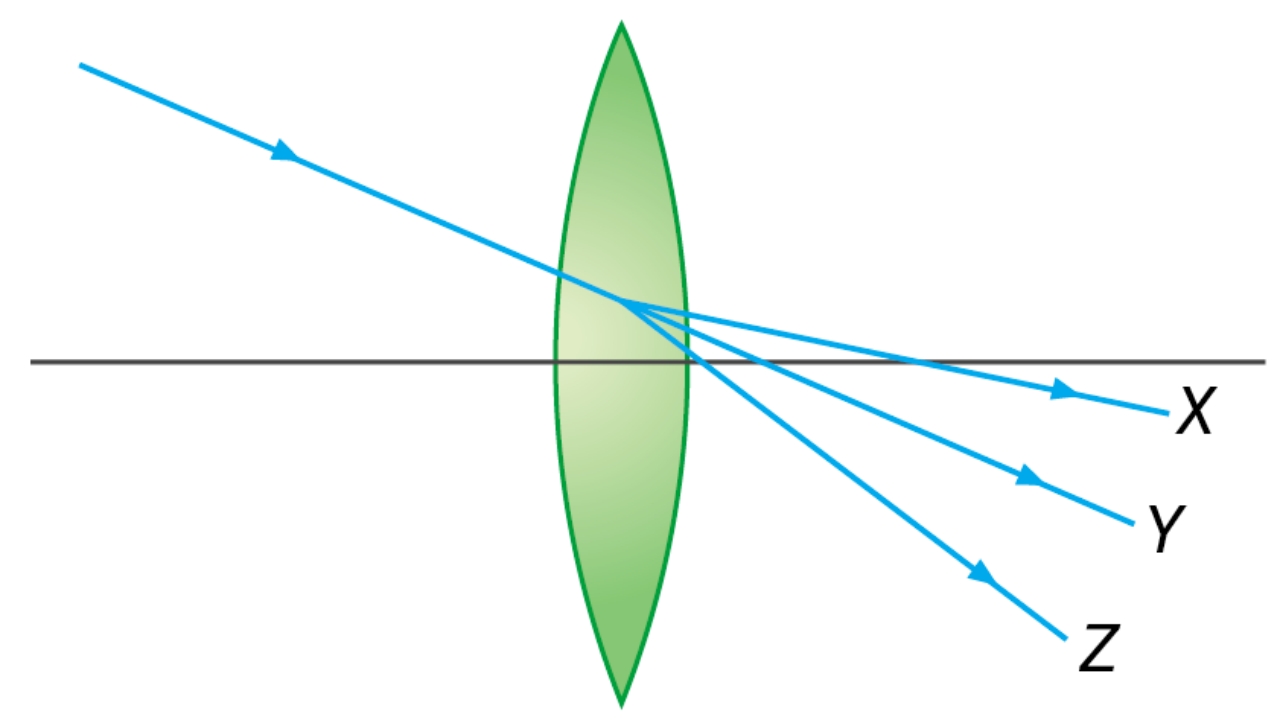
\includegraphics[width=0.65\linewidth]{assets/81xne89nu12.png}


    \end{figure}
\end{eg}

\begin{eg}
    光線斜射到一個凹透鏡上。哪一個最能代表光線的路徑,X、Y還是Z?\\A light ray is incident on a concave lens. Which one best represents the path of the light ray, X, Y or Z?
    \bigskip
    \begin{figure}
        \centering
        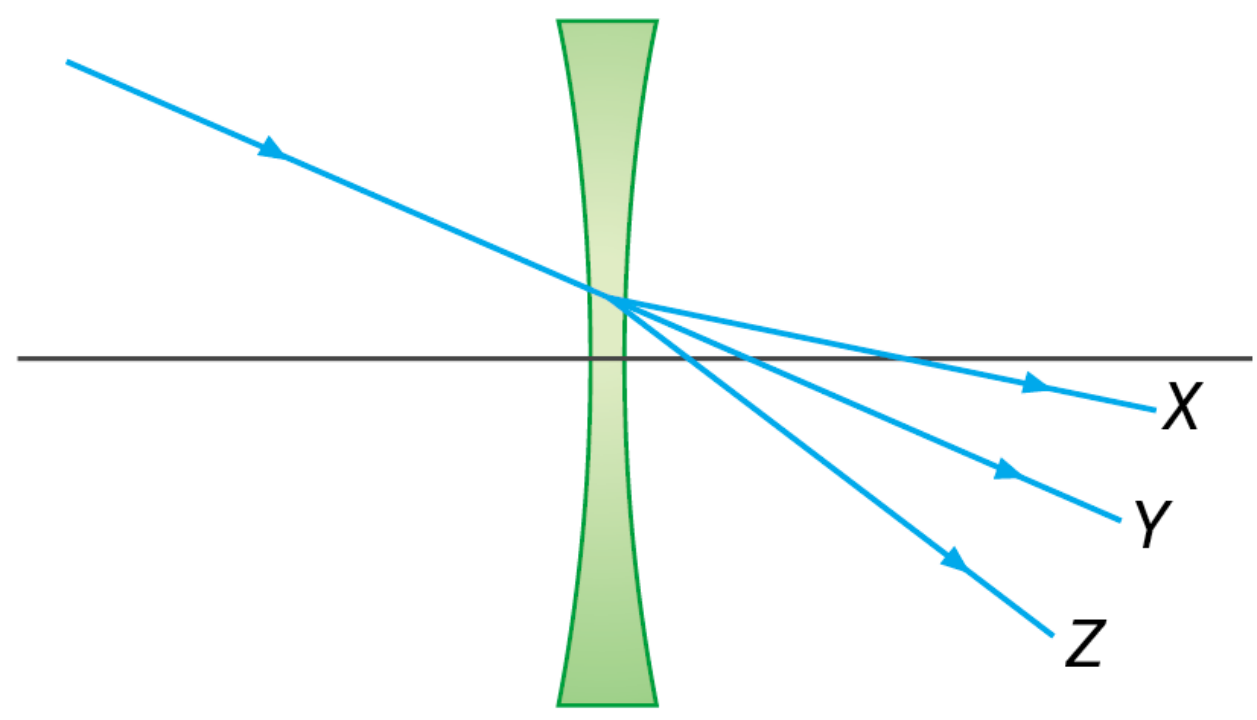
\includegraphics[width=0.65\linewidth]{assets/xn9eu19eud.png}


    \end{figure}
\end{eg}

\begin{eg}
    如果點F和F'代表凹透鏡的焦點,以下哪個光線圖正確地顯示了光線通過透鏡的路徑?\\If points F and F' represent the focal points of a concave lens, which of the following ray diagrams correctly shows the path of a light ray through the lens?
    \begin{tasks}[item-indent=2em,label-offset=0em,before-skip=0em,after-item-skip=0pt]
        (2)

        \task

        \topalign{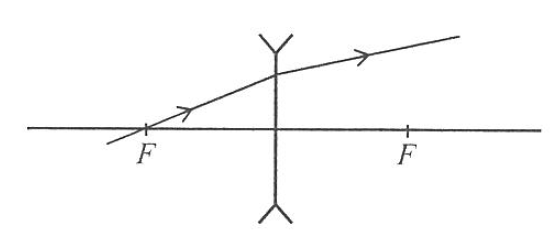
\includegraphics[width=.9\linewidth]{assets/xne98n1u982.png}}


        \task

        \topalign{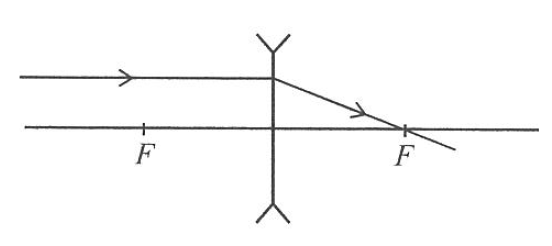
\includegraphics[width=.9\linewidth]{assets/d2un8xc2d3.png}}


        \task

        \topalign{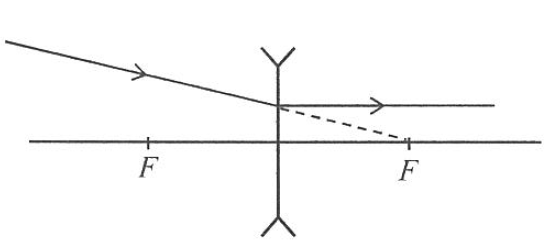
\includegraphics[width=.9\linewidth]{assets/x8n10u89e1ue82.png}}


        \task

        \topalign{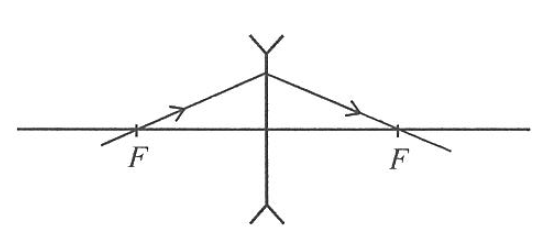
\includegraphics[width=.9\linewidth]{assets/x1n89ue8eu9812eage.png}}


    \end{tasks}
\end{eg}

\begin{eg}
    下列哪個(些)光線圖是正確的?\\Which of the following ray diagrams is/are correct?
    \begin{statements}
        [before-skip=0pt,after-item-skip=0pt,label-offset=1em,item-indent=2em] (2)
        \task
        \topalign{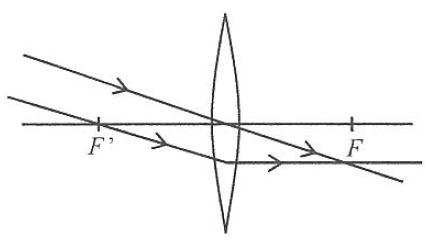
\includegraphics[width=.9\linewidth]{assets/x1nue9812.png}}


        \task
        \topalign{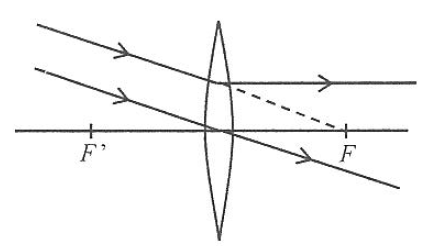
\includegraphics[width=.9\linewidth]{assets/xn1e891age.png}}

        \task
        \topalign{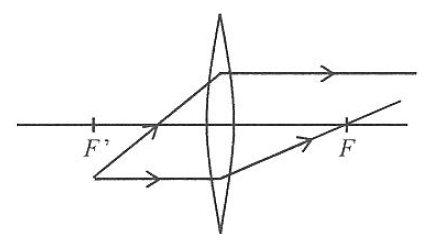
\includegraphics[width=.9\linewidth]{assets/x8n9u009e03298enx923.png}}



    \end{statements}
\end{eg}

% \begin{eg}
%     \begin{tasks}
%     \task 只有(1) \tab (1) only
%     \task 只有(1)和(2) \tab (1) and (2) only
%     \task 只有(2)和(3) \tab (2) and (3) only
%     \task (1), (2) 和 (3)\tab (1), (2) and (3)
% \end{tasks}  
% \end{eg}

% \begin{eg}
%     \begin{figure}
%         \centering
%         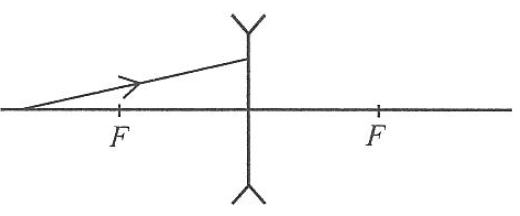
\includegraphics[width=0.5\linewidth]{assets/121n9812ue.png}


%     \end{figure}
%     一束光線射到一個凹透鏡上,F代表透鏡的焦點。以下哪個圖正確地顯示了出射光線的路徑?\\A ray of light is incident at a concave lens. F is the focus of the lens. Which of the following diagrams correctly shows the path of the emergent ray?
% \end{eg}

% \begin{eg}
%     \begin{tasks}[item-indent=1.7em,label-offset=0em] (2)
%         \task 
%     \topalign{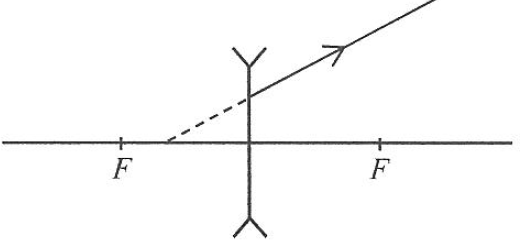
\includegraphics[width=1\linewidth]{assets/9nd8398ne9c8dc.png}}


%         \task 
%     \topalign{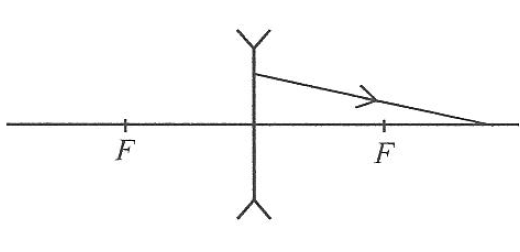
\includegraphics[width=1\linewidth]{assets/dqiwdniw0qdwq9id9wqd.png}}


%         \task 
%     \topalign{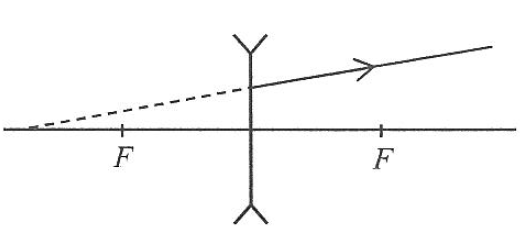
\includegraphics[width=1\linewidth]{assets/dnqwdwq90dqwd09wq.png}}


%         \task 
%     \topalign{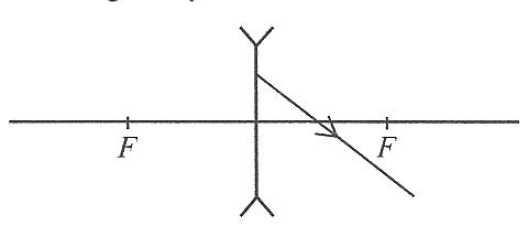
\includegraphics[width=1\linewidth]{assets/8n9eu89ewu98cew9.png}}



%     \end{tasks}
% \end{eg}

\begin{eg}
    一束光如圖入射一片透鏡。四條光線何者最可能是折射後的光路?\\A beam of light enters a lens as shown in the diagram. Which of the four rays is most likely the path after refraction?
    \begin{figure}
        \centering
        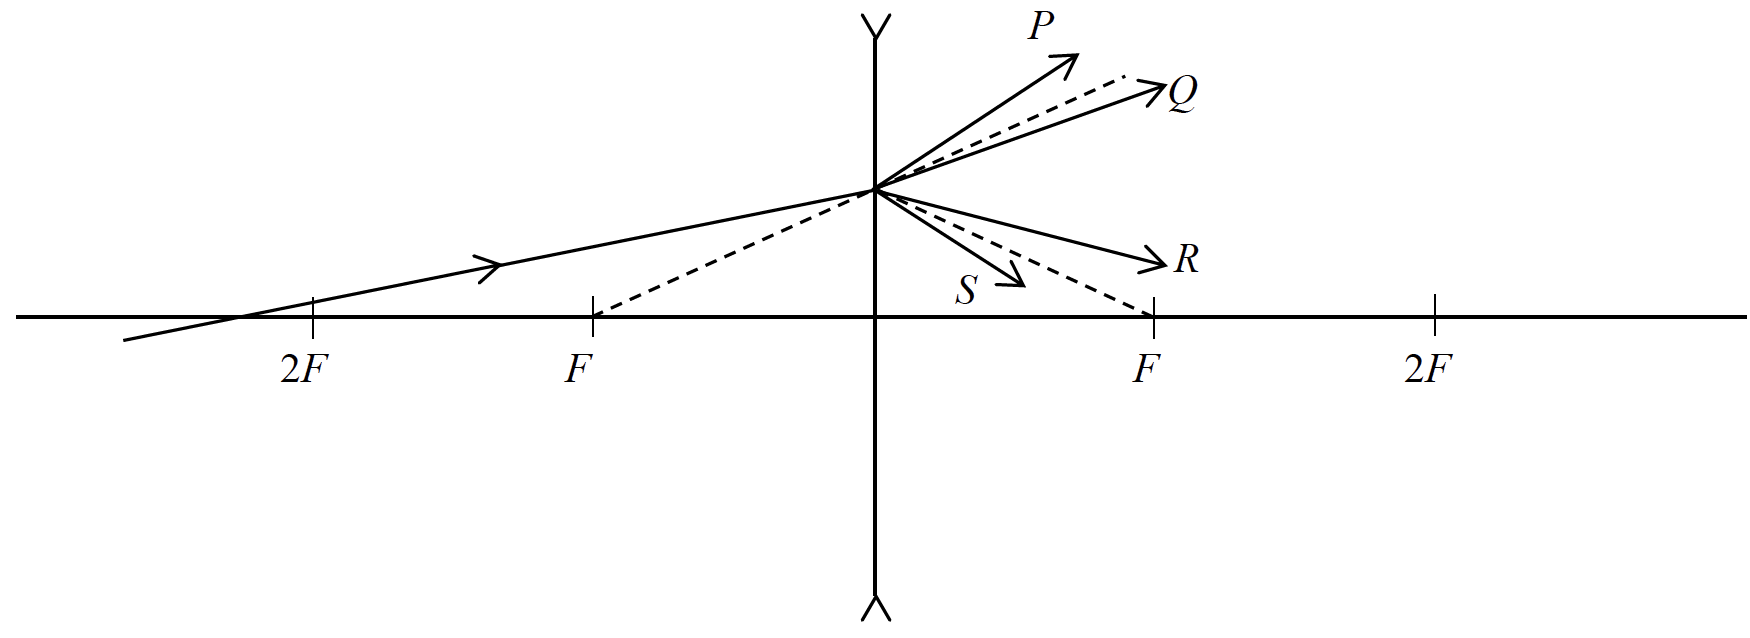
\includegraphics[width=1\linewidth]{assets/duqnu89n3.png}


    \end{figure}
    \begin{tasks}[before-skip=0em]
        (2)
        \task P
        \task Q
        \task R
        \task S
    \end{tasks}
\end{eg}

\begin{eg}
    \begin{figure}
        \centering
        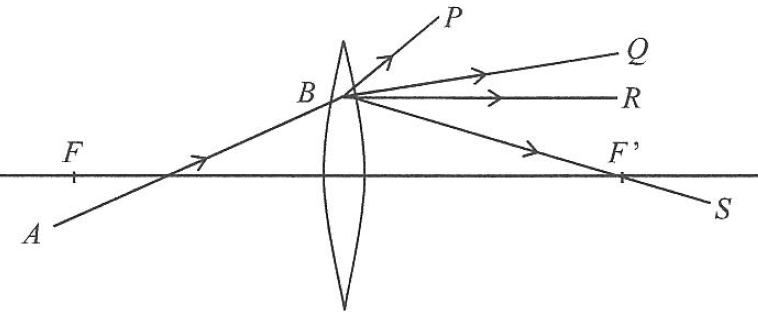
\includegraphics[width=0.6\linewidth]{assets/xn1e98u89.png}


    \end{figure}
    在上圖中,F、F'是凸透鏡的焦點,AB是入射光線。以下哪條光路最能表達出射光線?\\In the above diagram, F, F' are the foci of the convex lens and AB is an incident ray. Which of the following paths best represents the emergent ray?
    \begin{tasks}
        (2)
        \task P
        \task Q
        \task R
        \task S
    \end{tasks}
\end{eg}

\section{凸透鏡/凹透鏡的成像Image formed by convex/concave lens}

\begin{frame}{凸透鏡/凹透鏡的成像Image formed by convex/concave lens}
    \begin{itemize}
        \item 通常使用一條光線平行於光軸,和一條光線通過光心,來判斷成像的位置和大小。\\Usually, a ray parallel to the principal axis and a ray passing through the optical centre of the lens are drawn to determine the position and size of the image.
    \end{itemize}

\end{frame}

\begin{frame}{凸透鏡/凹透鏡的成像Image formed by convex/concave lens}
    \begin{figure}
        \centering
        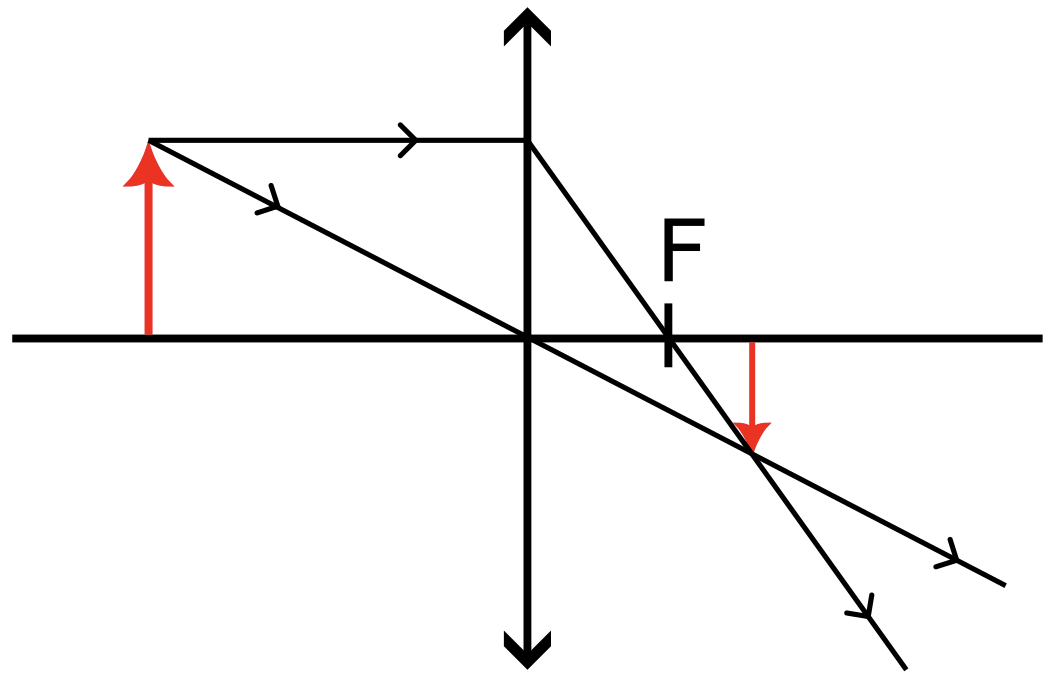
\includegraphics[width=0.75\linewidth]{assets/qxnuue8r923ge.png}


    \end{figure}

\end{frame}

\begin{frame}{凸透鏡/凹透鏡的成像Image formed by convex/concave lens}
    \begin{figure}
        \centering
        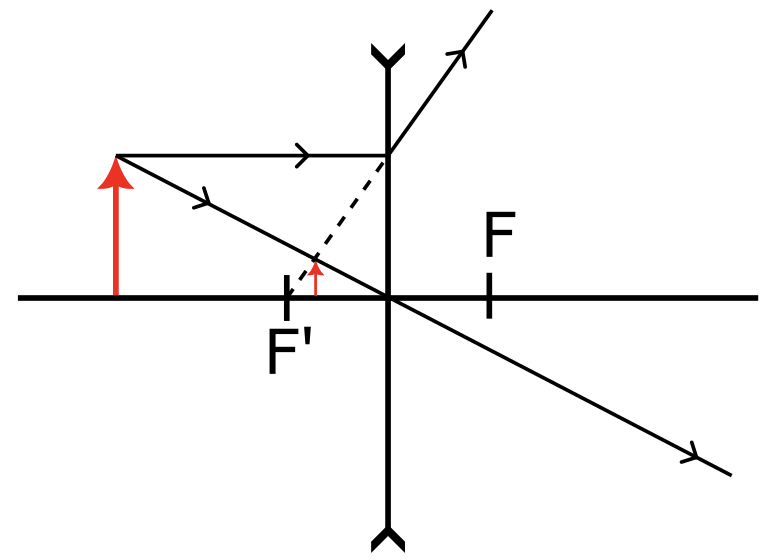
\includegraphics[width=0.75\linewidth]{assets/x1ni190necr4.png}


    \end{figure}

\end{frame}

\begin{frame}{凸透鏡成像Image formed by convex mirror}
    \begin{itemize}
        \item $u\approx\infty$
        \item 成像性質:倒立、縮小、實像
              \\Nature of image: inverted, diminished, real
    \end{itemize}
    \begin{figure}
        \centering
        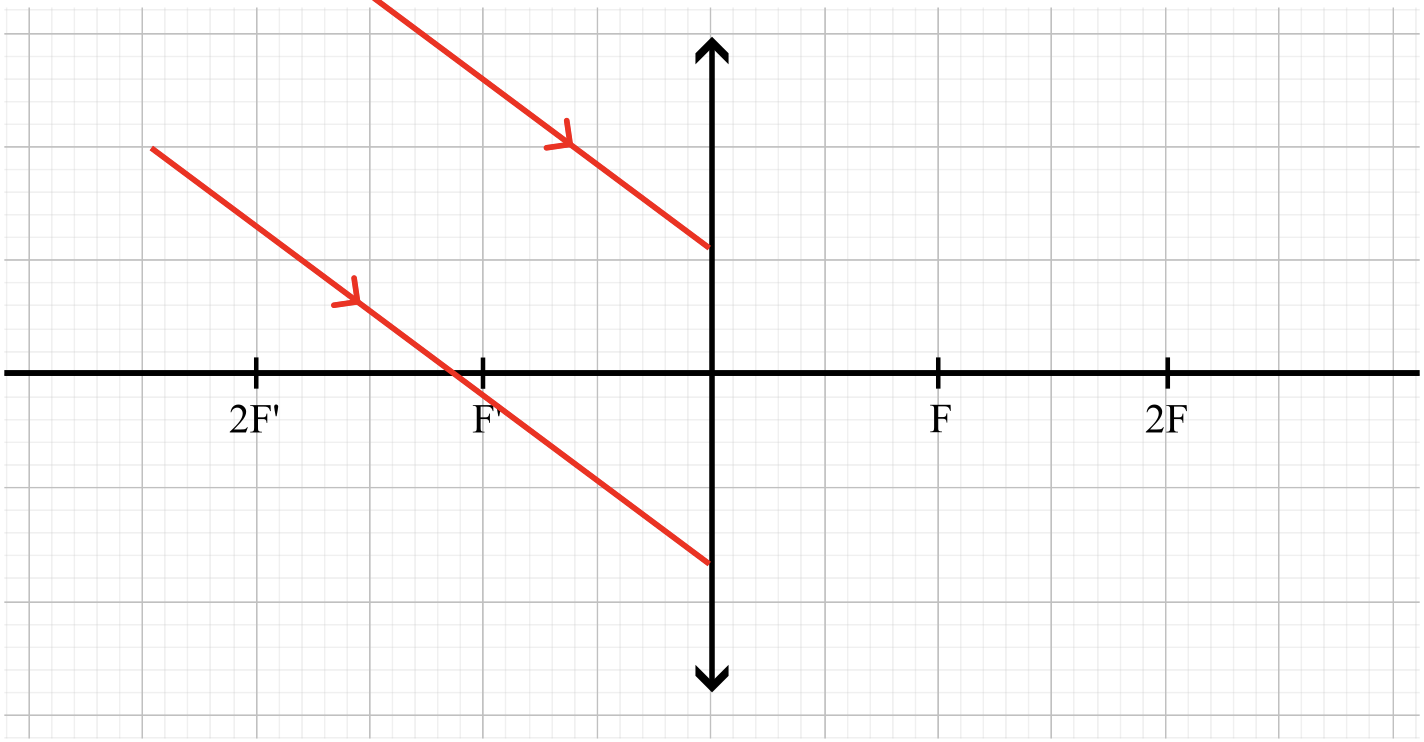
\includegraphics[width=1\linewidth]{assets/dn320un2d39u.png}


    \end{figure}
\end{frame}


% u>2F
\begin{frame}{凸透鏡成像Image formed by convex mirror}
    \begin{itemize}
        \item $u>2F\,'$
        \item 成像性質:倒立、縮小、實像
              \\Nature of image: inverted, diminished, real
    \end{itemize}
    \begin{figure}
        \centering
        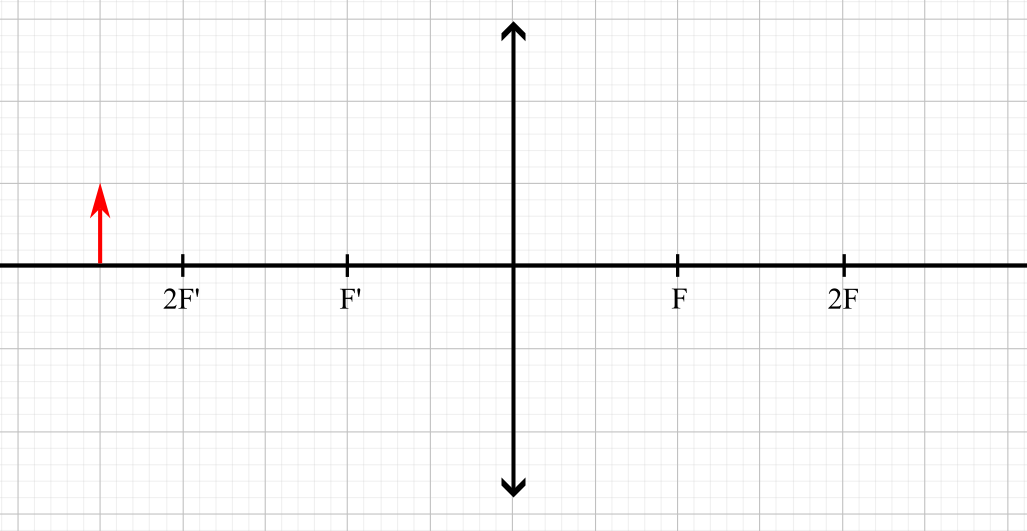
\includegraphics[width=1\linewidth]{assets/dqw0md9wdi.png}


    \end{figure}
\end{frame}

%u=2F
\begin{frame}{凸透鏡成像Image formed by convex mirror}
    \begin{itemize}
        \item $u=2F\,'$
        \item 成像性質:倒立、等大、實像
              \\Nature of image: inverted, same size, real
    \end{itemize}
    \begin{figure}
        \centering
        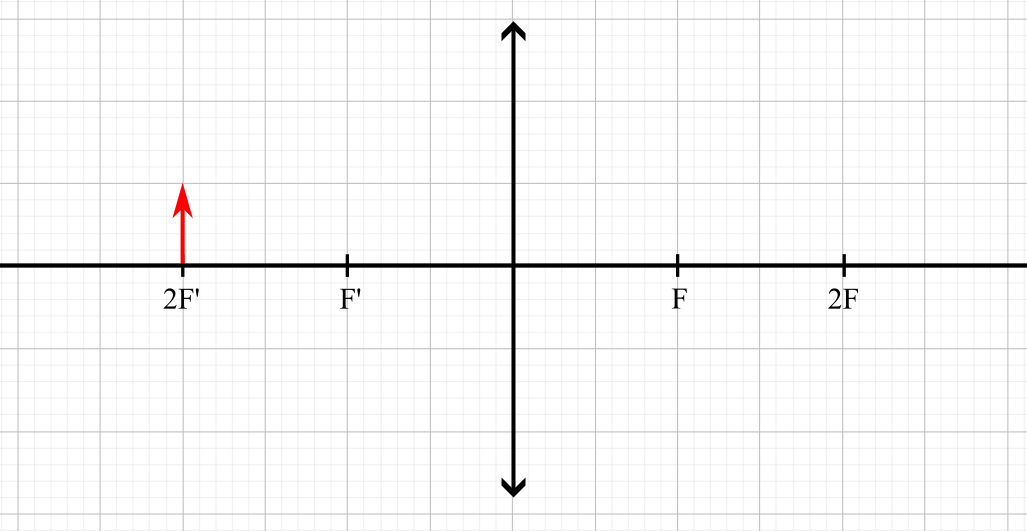
\includegraphics[width=1\linewidth]{assets/d8q9nwd8qwub8dnwq.png}


    \end{figure}
\end{frame}

\begin{frame}{凸透鏡成像Image formed by convex mirror}
    \begin{itemize}
        \item $F\,'<u<2F\,'$
        \item 成像性質:倒立、放大、實像
              \\Nature of image: inverted, magnified, real
    \end{itemize}
    \begin{figure}
        \centering
        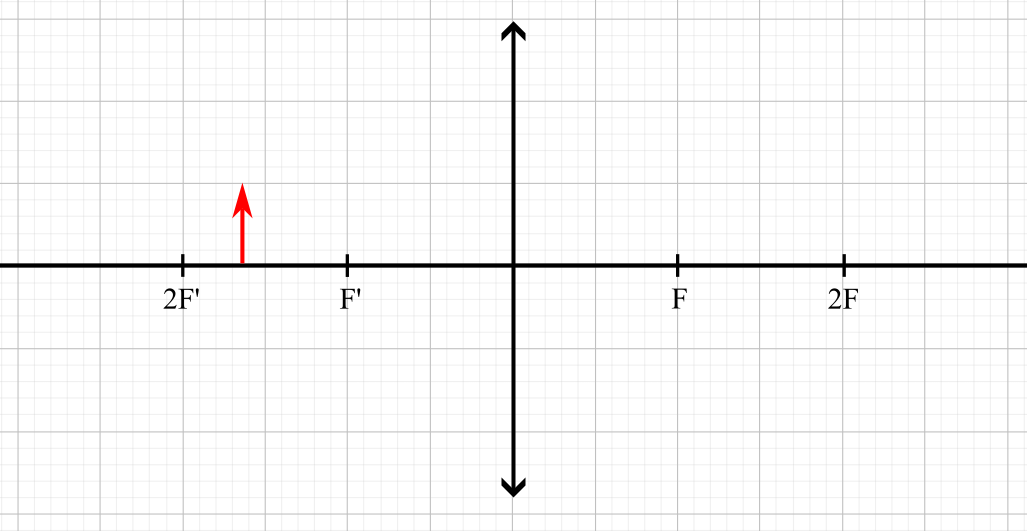
\includegraphics[width=1\linewidth]{assets/d9qi09mqwdqw.png}


    \end{figure}
\end{frame}


\begin{frame}{凸透鏡成像Image formed by convex mirror}
    \begin{itemize}
        \item $u=F\,'$
        \item 成像性質:不能判斷(只確定成像放大)
              \\Nature of image: undetermined (except magnified)
    \end{itemize}
    \begin{figure}
        \centering
        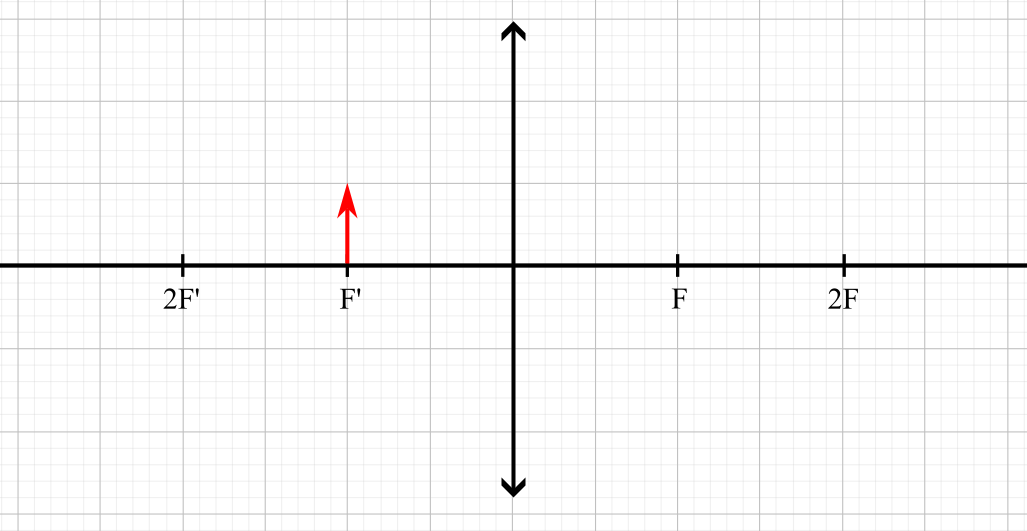
\includegraphics[width=1\linewidth]{assets/dqi0wqn9dqwd9age.png}


    \end{figure}
\end{frame}


\begin{frame}{凸透鏡成像Image formed by convex mirror}
    \begin{itemize}
        \item $u<F\,'$
        \item 成像性質:正立、放大、虛像
              \\Nature of image: erect, magnified, virtual
    \end{itemize}
    \begin{figure}
        \centering
        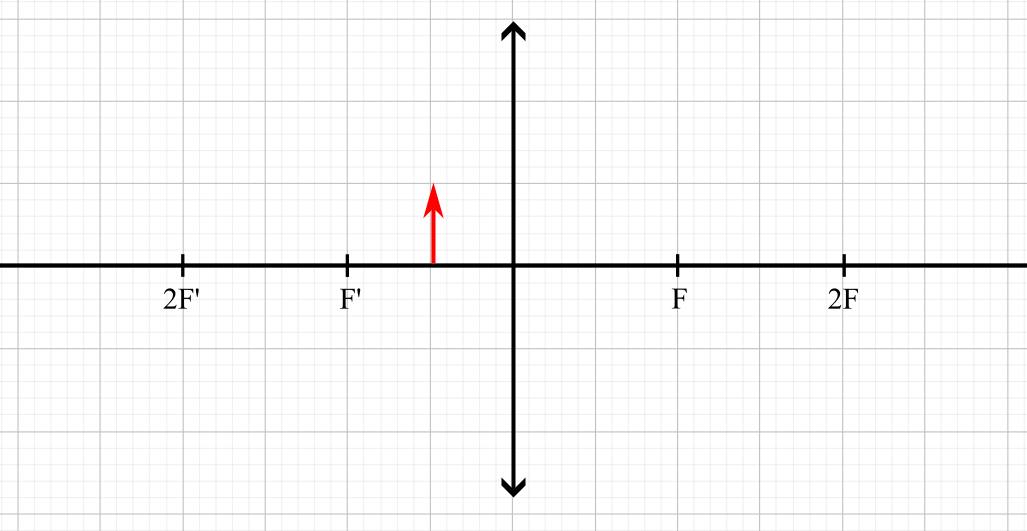
\includegraphics[width=1\linewidth]{assets/dqiwdwq09dwqe.png}


    \end{figure}
\end{frame}


\begin{frame}{凹透鏡成像Image formed by concave mirror}
    \begin{itemize}
        \item 成像性質:正立、縮小、虛像
              \\Nature of image: erect, diminished, virtual
    \end{itemize}
    \begin{figure}
        \centering
        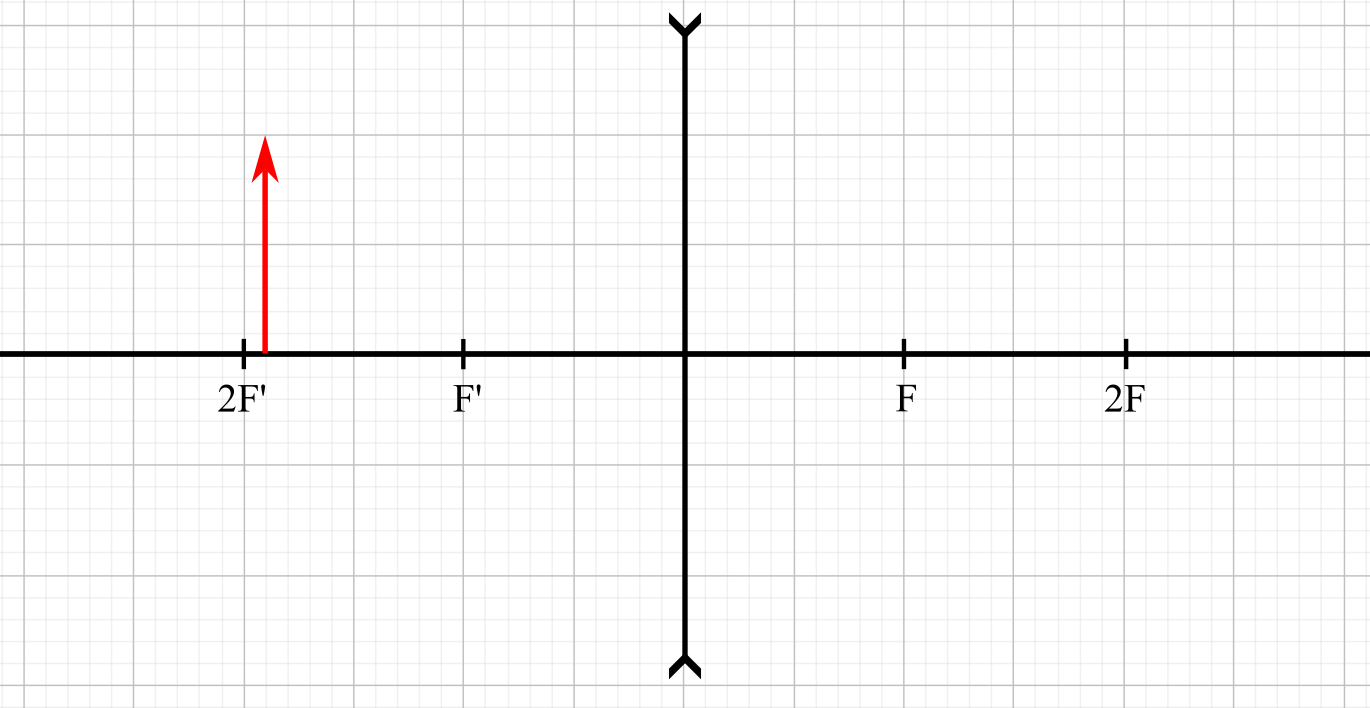
\includegraphics[width=1\linewidth]{assets/dqdnq90wdwq.png}


    \end{figure}
\end{frame}

\begin{frame}{凹透鏡成像Image formed by concave mirror}
    \begin{itemize}
        \item 成像性質:正立、縮小、虛像
              \\Nature of image: erect, diminished, virtual
    \end{itemize}
    \begin{figure}
        \centering
        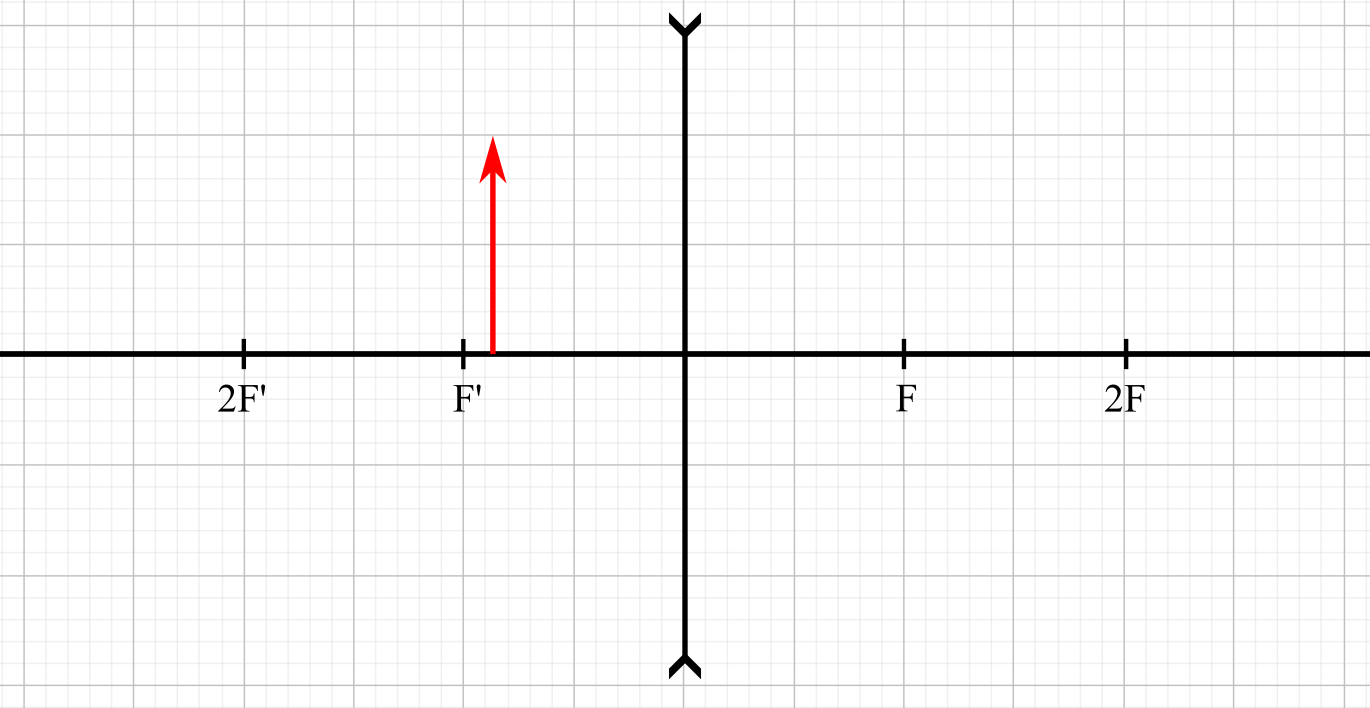
\includegraphics[width=1\linewidth]{assets/d9qwni0d9nwqdqw.png}
    \end{figure}
\end{frame}

\begin{frame}{凹透鏡成像Image formed by concave mirror}
    \begin{itemize}
        \item 成像性質:正立、縮小、虛像
              \\Nature of image: erect, diminished, virtual
    \end{itemize}
    \begin{figure}
        \centering
        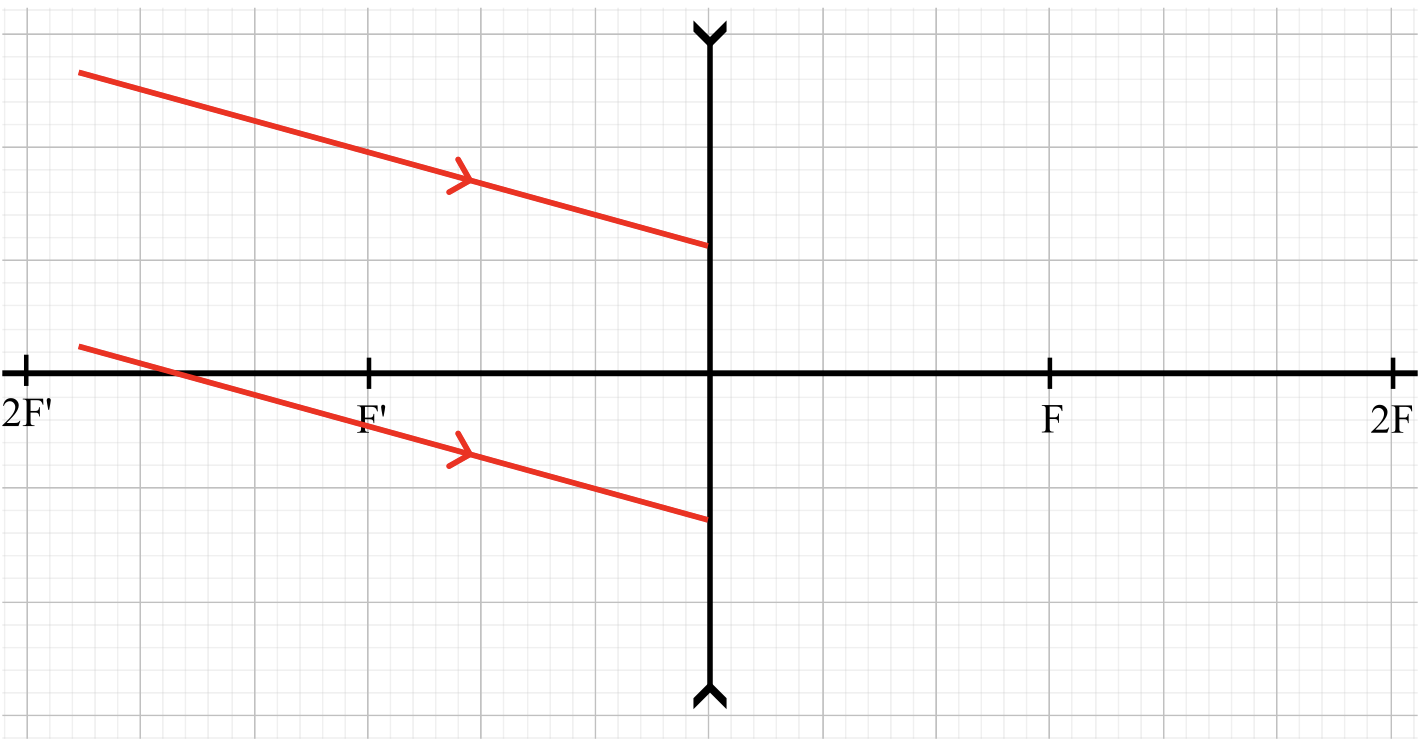
\includegraphics[width=1\linewidth]{assets/nud98u2dn32.png}


    \end{figure}
\end{frame}

\begin{frame}{凸透鏡成像Images of convex lens}
    \begin{figure}
        \centering
        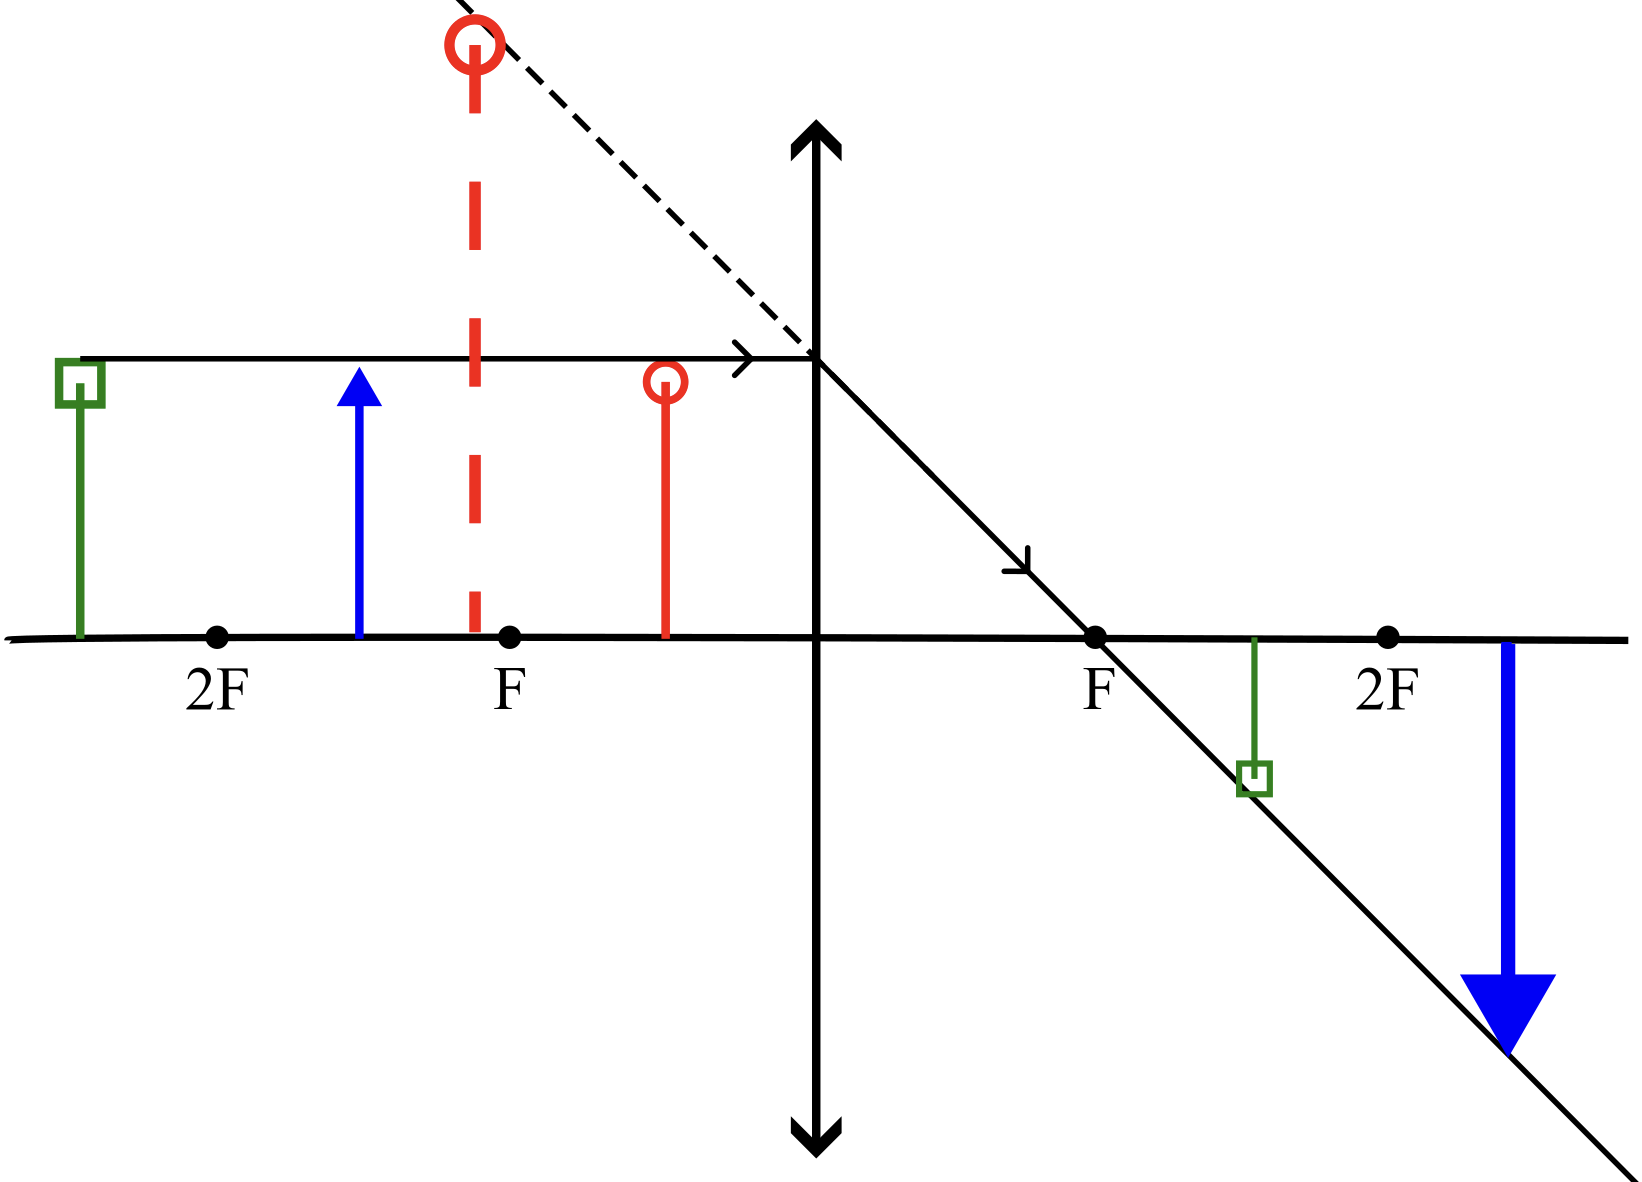
\includegraphics[width=1\linewidth]{assets/dqdqwdund3.png}


    \end{figure}
\end{frame}

\begin{frame}{凹透鏡成像Images of concave lens}
    \begin{figure}
        \centering
        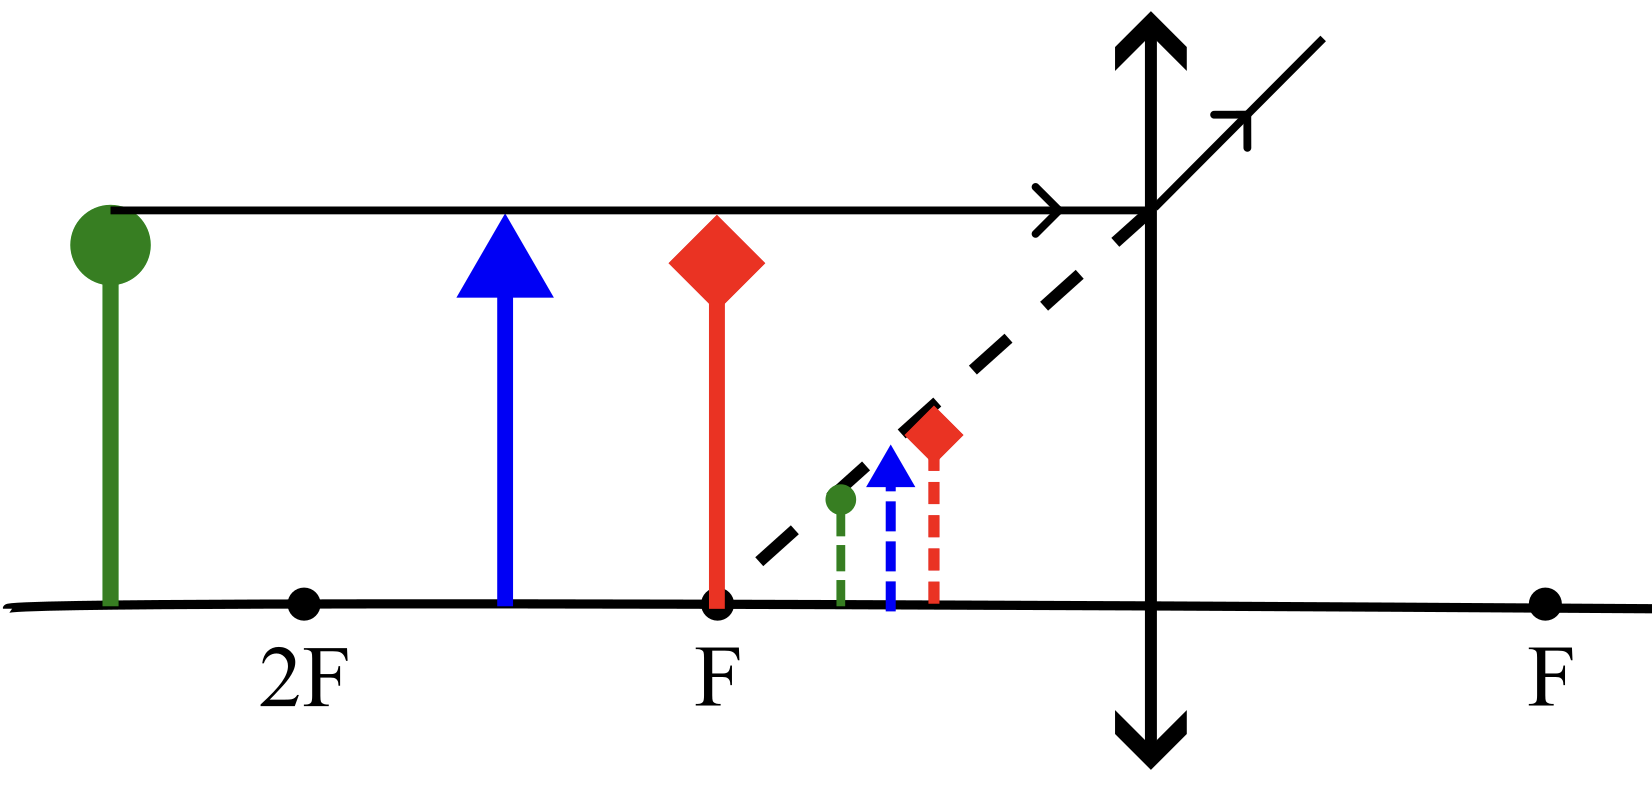
\includegraphics[width=1\linewidth]{assets/jdnd3d23dc.png}


    \end{figure}
\end{frame}
% \begin{frame}{小結Summary}
%     For convex lens, when object distance $>$ focal length, real and inverted image. When object distance 
% \end{frame}

% \begin{frame}{例題Example}
%     If refractive index increases, what happens to the image formed?
%     Refractive index x
% \end{frame}

\begin{eg}
    以下哪個/些光線圖可能正確?\\Which of the following ray diagram(s) might be correct?
    \begin{statements}
        [item-indent=2em,label-offset=0.5em,before-skip=0em](2)
        \task
        \topalign{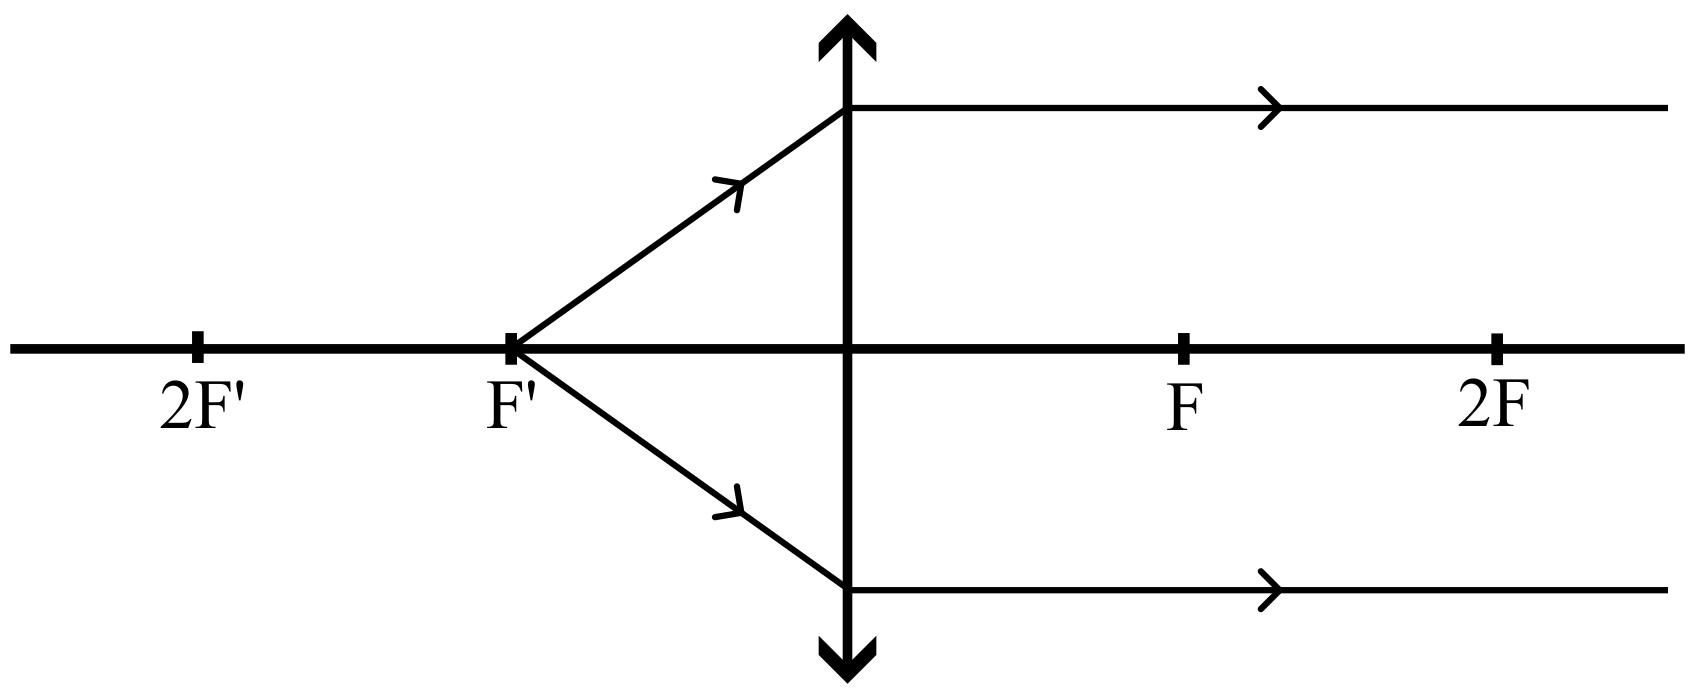
\includegraphics[width=1\linewidth]{assets/xn9812eage.png}}
        \task
        \topalign{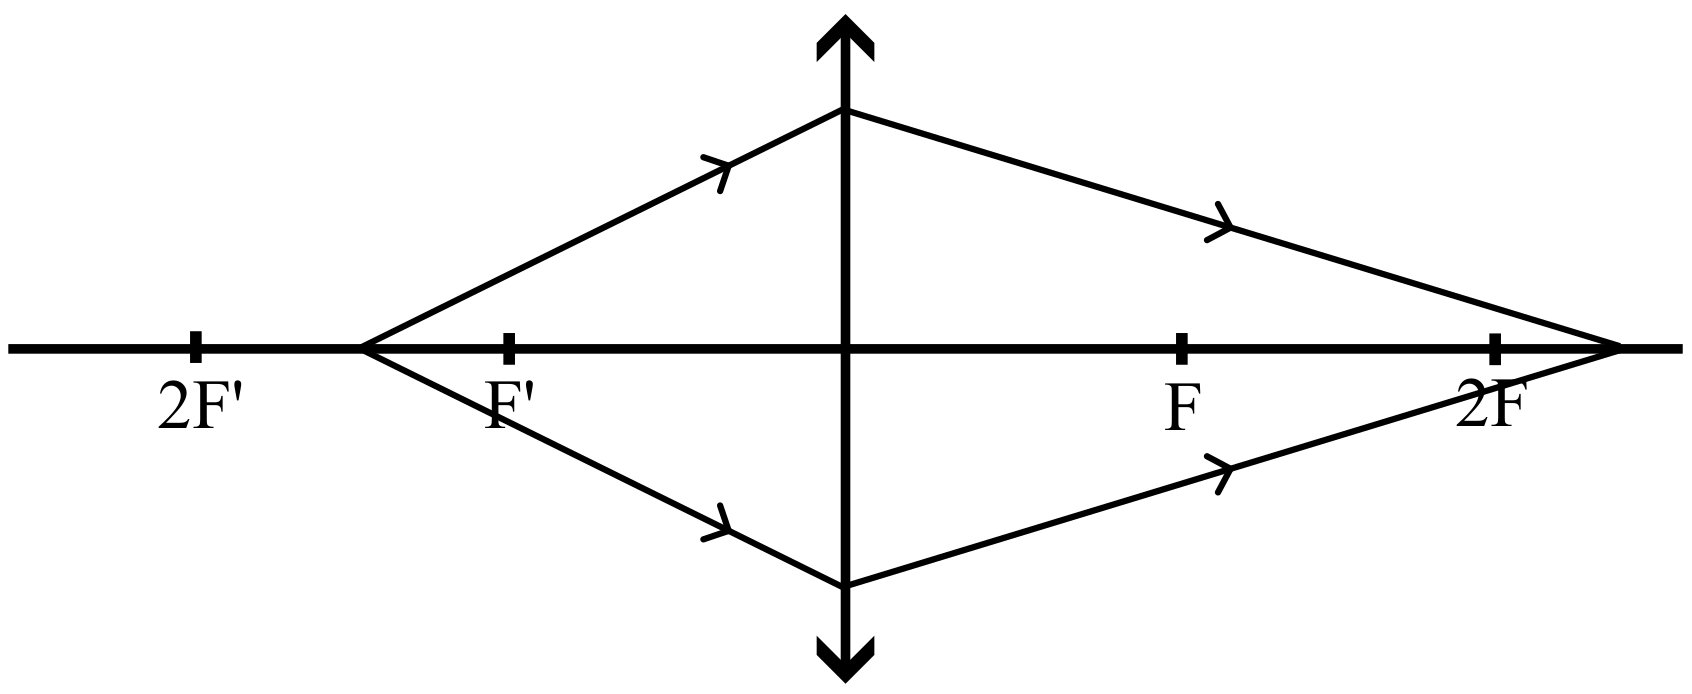
\includegraphics[width=\linewidth]{assets/dmdi90qwind09qw.png}}
        \task
        \topalign{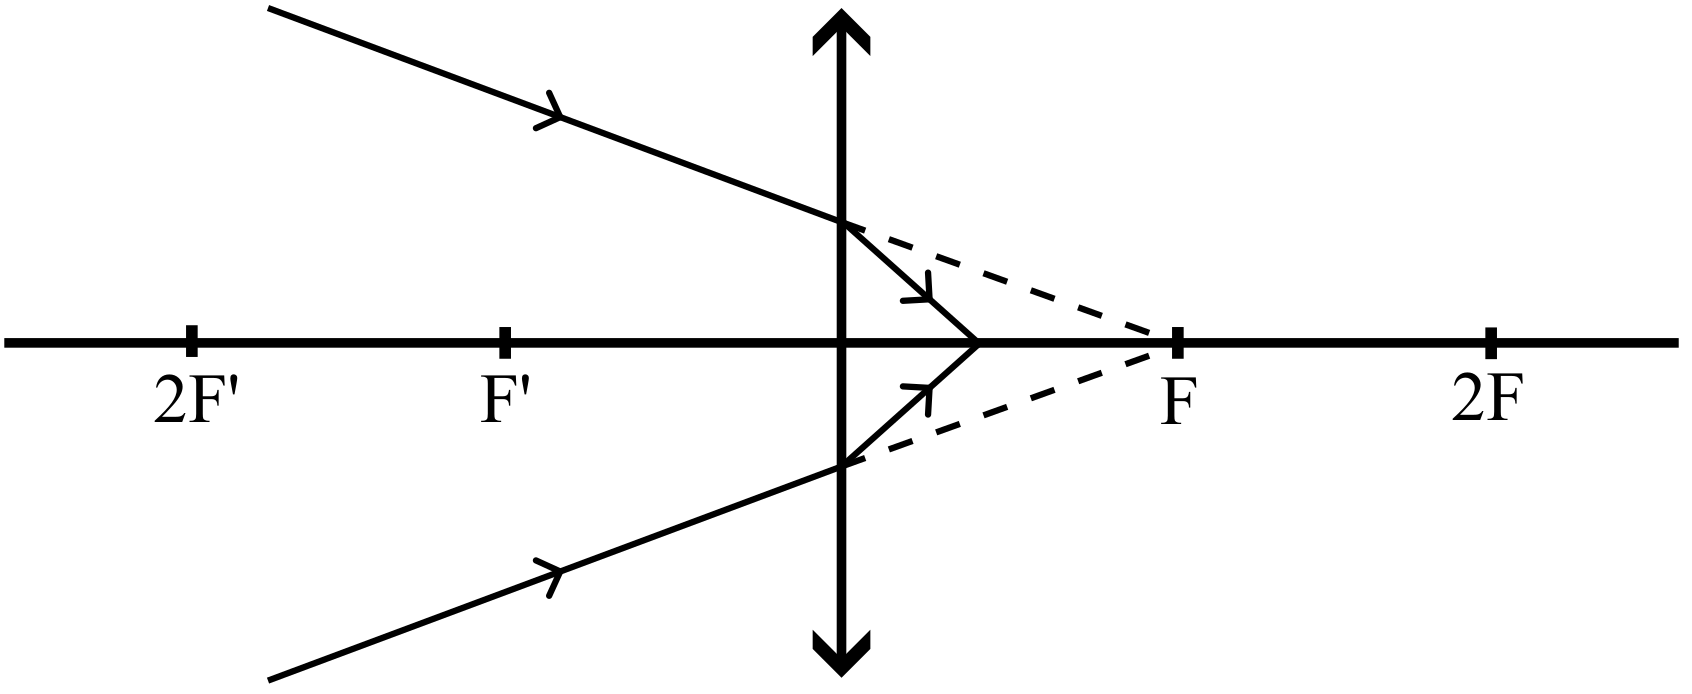
\includegraphics[width=\linewidth]{assets/idq9wid90qmage.png}}

    \end{statements}
\end{eg}


\begin{eg}
    以下哪個/些光線圖可能正確?\\Which of the following ray diagram(s) might be correct?
    \begin{statements}
        [item-indent=2em,label-offset=0.5em,before-skip=0em](2)
        \task
        \topalign{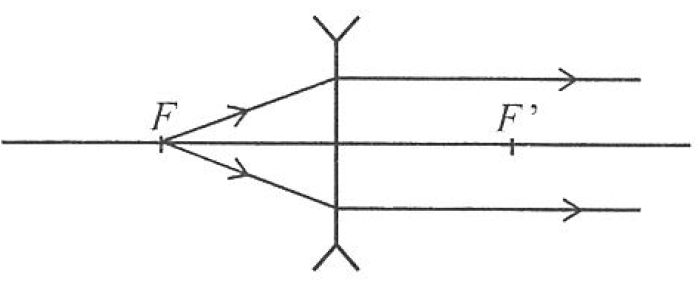
\includegraphics[width=1\linewidth]{assets/dqwd09iqn.png}}
        % \task 
        % \topalign{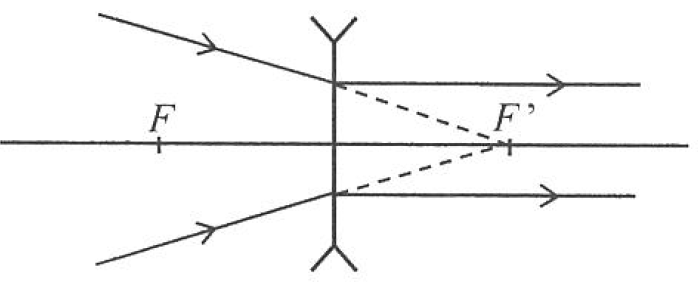
\includegraphics[width=1\linewidth]{assets/dqun89qwd21d.png}}
        \task
        \topalign{\includegraphics[width=1\linewidth]{assets/dw9ijn3209d29f3.png}}

        \task
        \topalign{
            \includegraphics[width=1\linewidth]{assets/dqwi09qmwdqw.png}
        }



    \end{statements}
\end{eg}

\begin{eg}
    以下哪個/些光線圖可能正確?\\Which of the following ray diagram(s) might be correct?
    \begin{statements}
        [item-indent=2em,label-offset=0.5em,before-skip=0em](2)
        \task
        \topalign{\includegraphics[width=.8\linewidth]{assets/dqwqjmdiow.png}}
        \task
        \topalign{\includegraphics[width=.8\linewidth]{assets/dq0w9diwq9dnwq.png}}
        \task
        \topalign{\includegraphics[width=.8\linewidth]{assets/d9uqw89q0nwq.png}}

    \end{statements}
\end{eg}



\begin{eg}
    L是一面未知透鏡。哪一點(P 或 Q)可以是它的焦點?\\L is an unknown lens, which point, P or Q, could be focal point of the lens?
    \begin{figure}
        \centering
        \includegraphics[width=0.9\linewidth]{assets/djewdineuwdge.png}


    \end{figure}
\end{eg}
\begin{eg}
    L是一面未知透鏡。哪一點(P 或 Q)可以是它的焦點?\\L is an unknown lens, which point, P or Q, could be focal point of the lens?
    \begin{figure}
        \centering
        \includegraphics[width=0.9\linewidth]{assets/djewdineuwdge.png}


    \end{figure}
\end{eg}


\begin{eg}
    \begin{figure}
        \centering
        \includegraphics[width=0.6\linewidth]{assets/9nd832d.png}


    \end{figure}
    上方圖示顯示了一個物體OP放在一個凸透鏡前面。以下哪一個最能顯示它的像?\\The figure above shows an object OP placed in front of a convex lens. Which of the following best shows its image?
    \begin{tasks}
        (2)
        \task IQ
        \task IR
        \task IS
        \task IT
    \end{tasks}
\end{eg}

\begin{eg}
    \begin{figure}
        \centering
        \includegraphics[width=0.75\linewidth]{assets/dewdn9u823.png}


    \end{figure}
\end{eg}

\begin{eg}
    上圖所示,一個物體放在一個會聚透鏡前。圖中顯示的四束光線均來自物體。\\An object is placed in front of a converging lens as shown in the figure. The four light rays shown come from the object.
    \begin{itemize}
        \item [(a)] 在圖中完成光線的路徑並找出影像的位置。\\Complete the ray paths in the figure and locate the image.
        \item [(b)] 求透鏡的焦距。\\Find the focal length of the lens.
    \end{itemize}

\end{eg}

\begin{eg}
    \begin{figure}
        \centering
        \includegraphics[width=0.95\linewidth]{assets/odijdoid.png}


    \end{figure}

\end{eg}

\begin{eg}
    \begin{itemize}
        \item [(a)] 圖中是何種透鏡?解釋你的答案。\\What kind of lens is it? Explain your answer.\vspace{3cm}
        \item [(b)] 寫出透鏡的焦距。\\ Write down the focal length of the lens.\vspace{1cm}
        \item [(c)] 在上圖中完成y的光線穿過透鏡的路徑。\\Complete the ray path when ray y passes through the lens.
    \end{itemize}
\end{eg}

\begin{eg}
    \begin{figure}
        \centering
        \includegraphics[width=1\linewidth]{assets/89dnu832d9832d98un32.png}
    \end{figure}
\end{eg}

\begin{eg}
    \begin{itemize}
        \setlength{\itemsep}{0.8em}
        \item [(a)] 畫一條適當的光線以決定B的像位置(標記為B')。\\Draw a suitable line so as to locate the image of B (denote as B').
        \item [(b)] 標記物件AB的像A'B'。\\Mark the image A'B' of object AB.
        \item [(c)] 畫出\textbf{一條}適當的光線,在圖示上標記並找出透鏡L的主焦點F,同時寫出焦距f。\\By drawing \textbf{ONE} suitable ray, locate and mark the principal focus F of the lens L on your diagram and find the focal length f.
    \end{itemize}
\end{eg}

















































\end{document}